\section{Pendahuluan}
\subsection{Latar Belakang}

Pada modul pertama, praktikan mempelajari penggunaan osiloskop dan function generator.
Proses pengolahan sinyal digital, peralatan pengukuran dan pengujian sangatlah penting untuk memastikan bahwa sinyal yang diolah telah sesuai dengan spesifikasi yang diinginkan. Dalam konteks ini, osiloskop dan function generator merupakan peralatan yang sangat fundamental.
\\\\
Osiloskop merupakan alat ukur elektronik yang digunakan untuk melakukan visualisasi sinyal listrik dalam bentuk gelombang. Dengan osiloskop, kita dapat mengamati perubahan tegangan seiring waktu, yang sangat berguna untuk menganalisis karakteristik sinyal dalam rangkaian elektronik.
Osiloskop memungkinkan pengguna untuk: mengukur frekuensi dan periode sinyal, mengamati bentuk gelombang dan mendeteksi distorsi atau noise, mengukur tegangan puncak ke puncak (Vpp) dan tegangan rata-rata, dan menganalisis hubungan fasa antara dua sinyal.
\\\\
Function generator adalah alat yang digunakan untuk menghasilkan berbagai bentuk gelombang listrik, seperti gelombang sinus, persegi, segitiga, dan gigi gergaji. 
Function generator sangat berguna dalam pengujian dan pengembangan rangkaian elektronik karena memungkinkan pengguna untuk: menghasilkan sinyal dengan frekuensi dan amplitudo yang dapat diatur, menguji respons rangkaian terhadap berbagai bentuk gelombang, dan mensimulasikan kondisi operasi yang berbeda dalam rangkaian.

\subsection{Maksud dan Tujuan}
Mengetahui dan memahami dasar penggunaan osiloskop dan function generator.

\subsection{Hasil yang diharapkan}
Dapat memahami dasar penggunaan osiloskop dan function generator.

%===========================================================%
\section{Tugas Pendahuluan}
\begin{enumerate}
\item Buatlah
\end{enumerate}

%===========================================================%
\section{Alat dan Bahan}
\begin{itemize}[label=$\bullet$, itemsep=-1pt, leftmargin=*]
	\item Function generator
	\item Osiloskop
	\item Kabel probe
\end{itemize}

%===========================================================%
\section{Jangka Waktu Pelaksanaan}
Pemahaman dan konfigurasi 30 menit.

%===========================================================%

\section{Proses dan Tahapan Konfigurasi}
%======================PERCOBAAN 1==========================%
\subsection{Percobaan 1}
\begin{center}

	\textbf{Konfigurasi Osiloskop}
	\begin{enumerate}
		\item Hubungkan kabel power ke osiloskop, lalu tekan tombol power untuk menyalakan Osiloskop. 
			\begin{figure}[H]
				\centering
				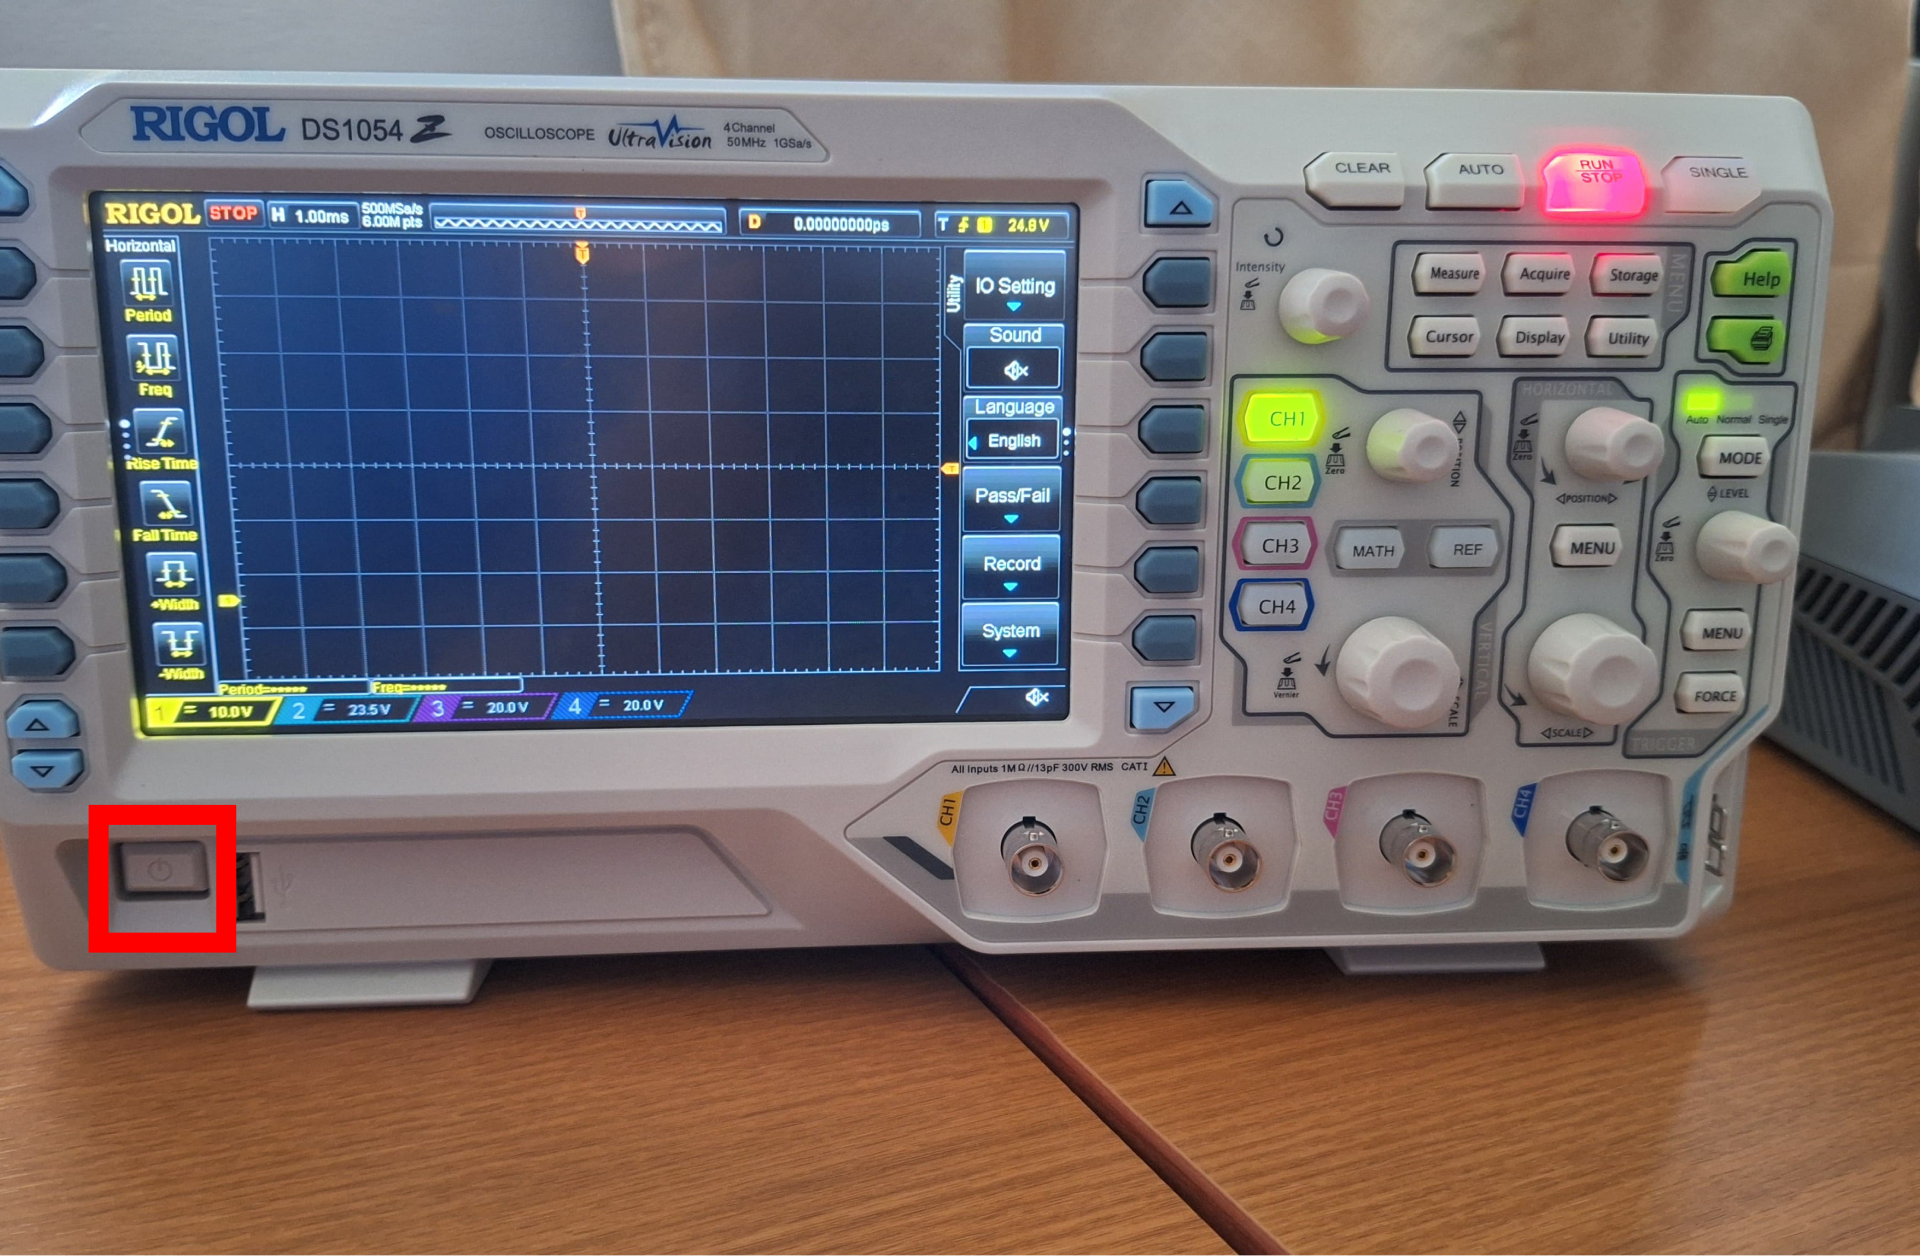
\includegraphics[width=0.8\linewidth]{P1/img/per 1/step 1.png}
				\caption{Step 1}
				\label{fig:Step 1(Group 7)}
			\end{figure}

		\item Hubungkan kabel probe pada channel 1.
			\begin{figure}[H]
				\centering
				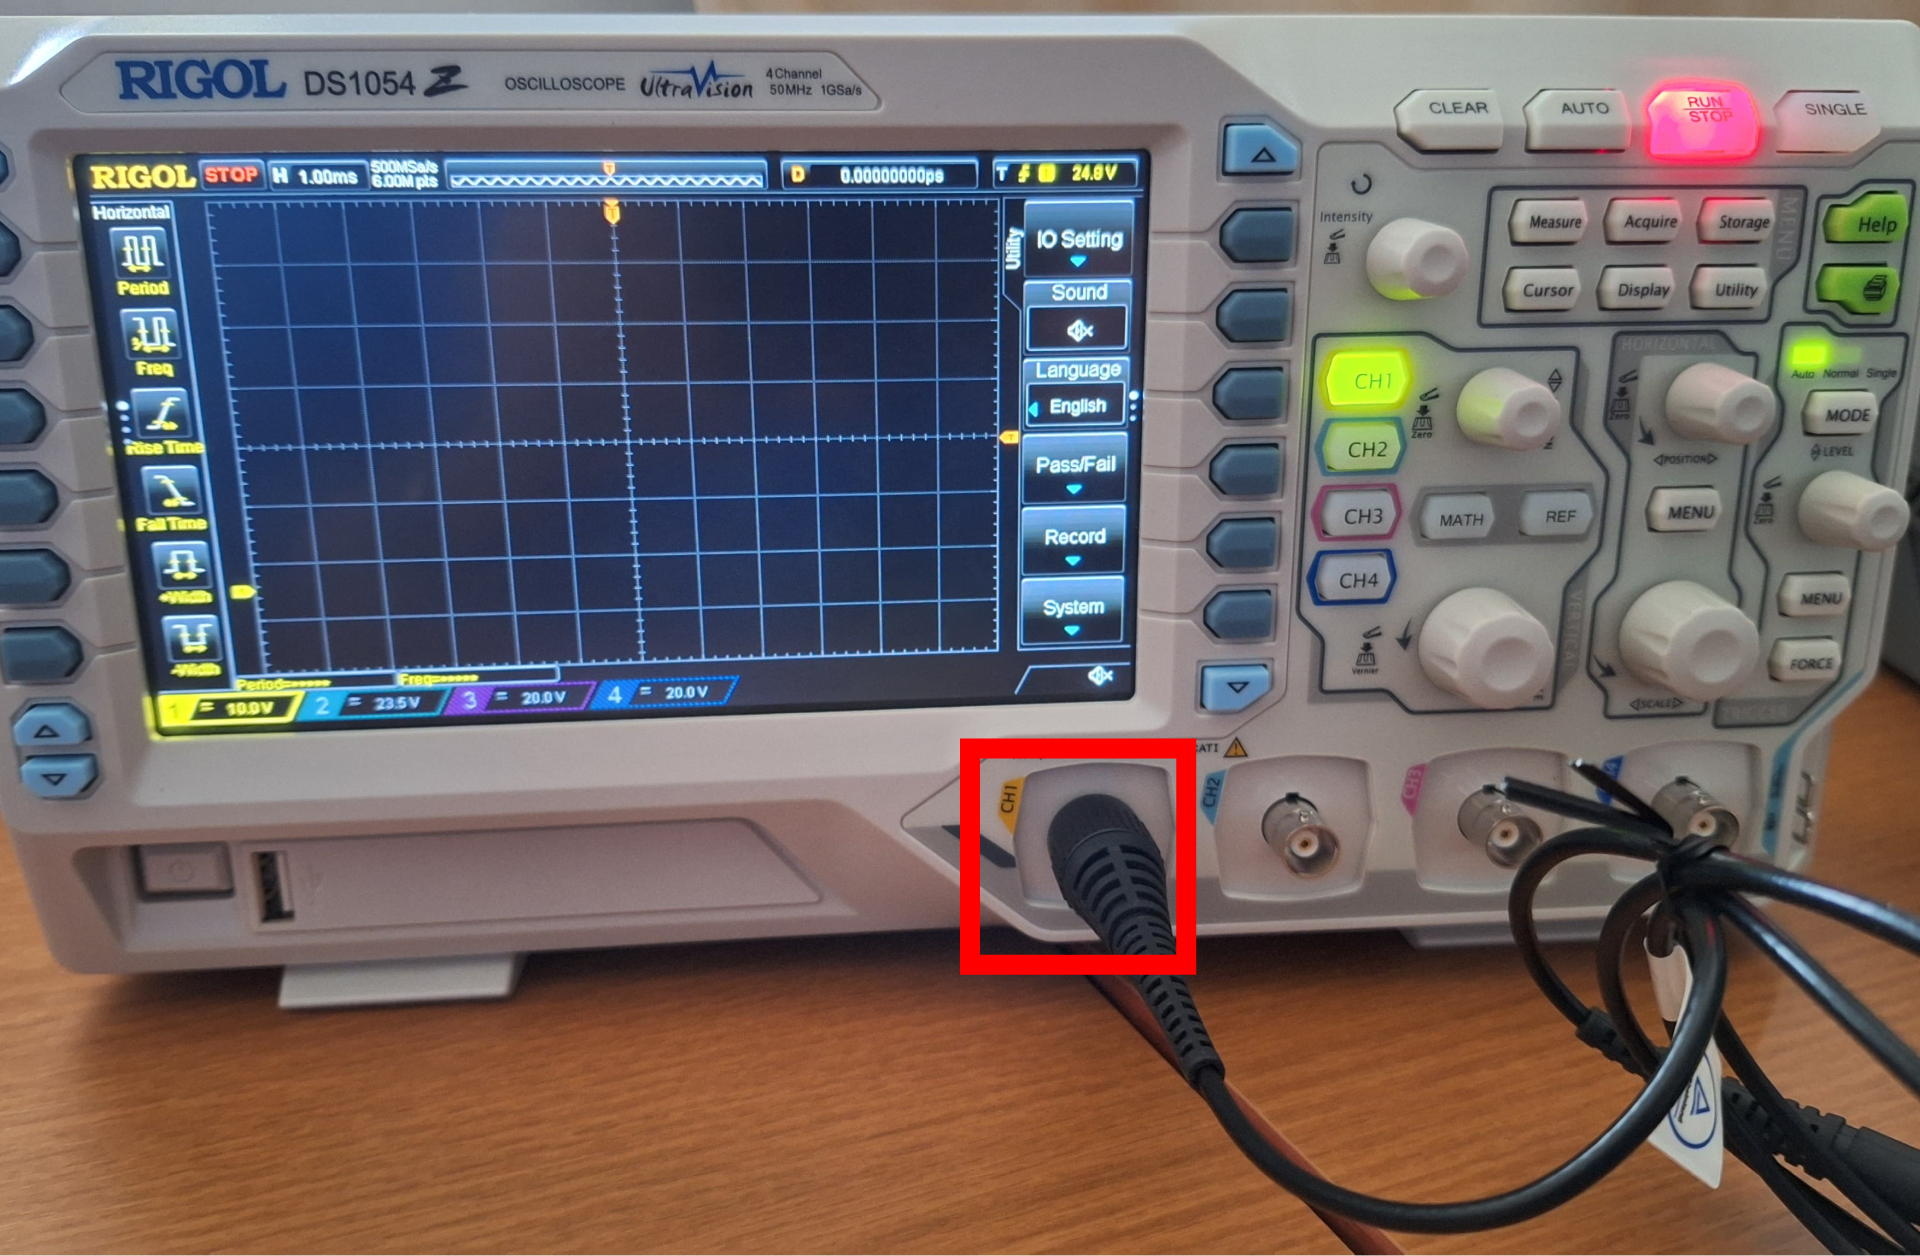
\includegraphics[width=0.8\linewidth]{P1/img/per 1/step 2.png}
				\caption{Step 2}
				\label{fig:Step 2(Group 14)}
			\end{figure}

		\item Hubungkan probe pengait pada pengkalibrasi osiloskop.
			\begin{figure}[H]
				\centering
				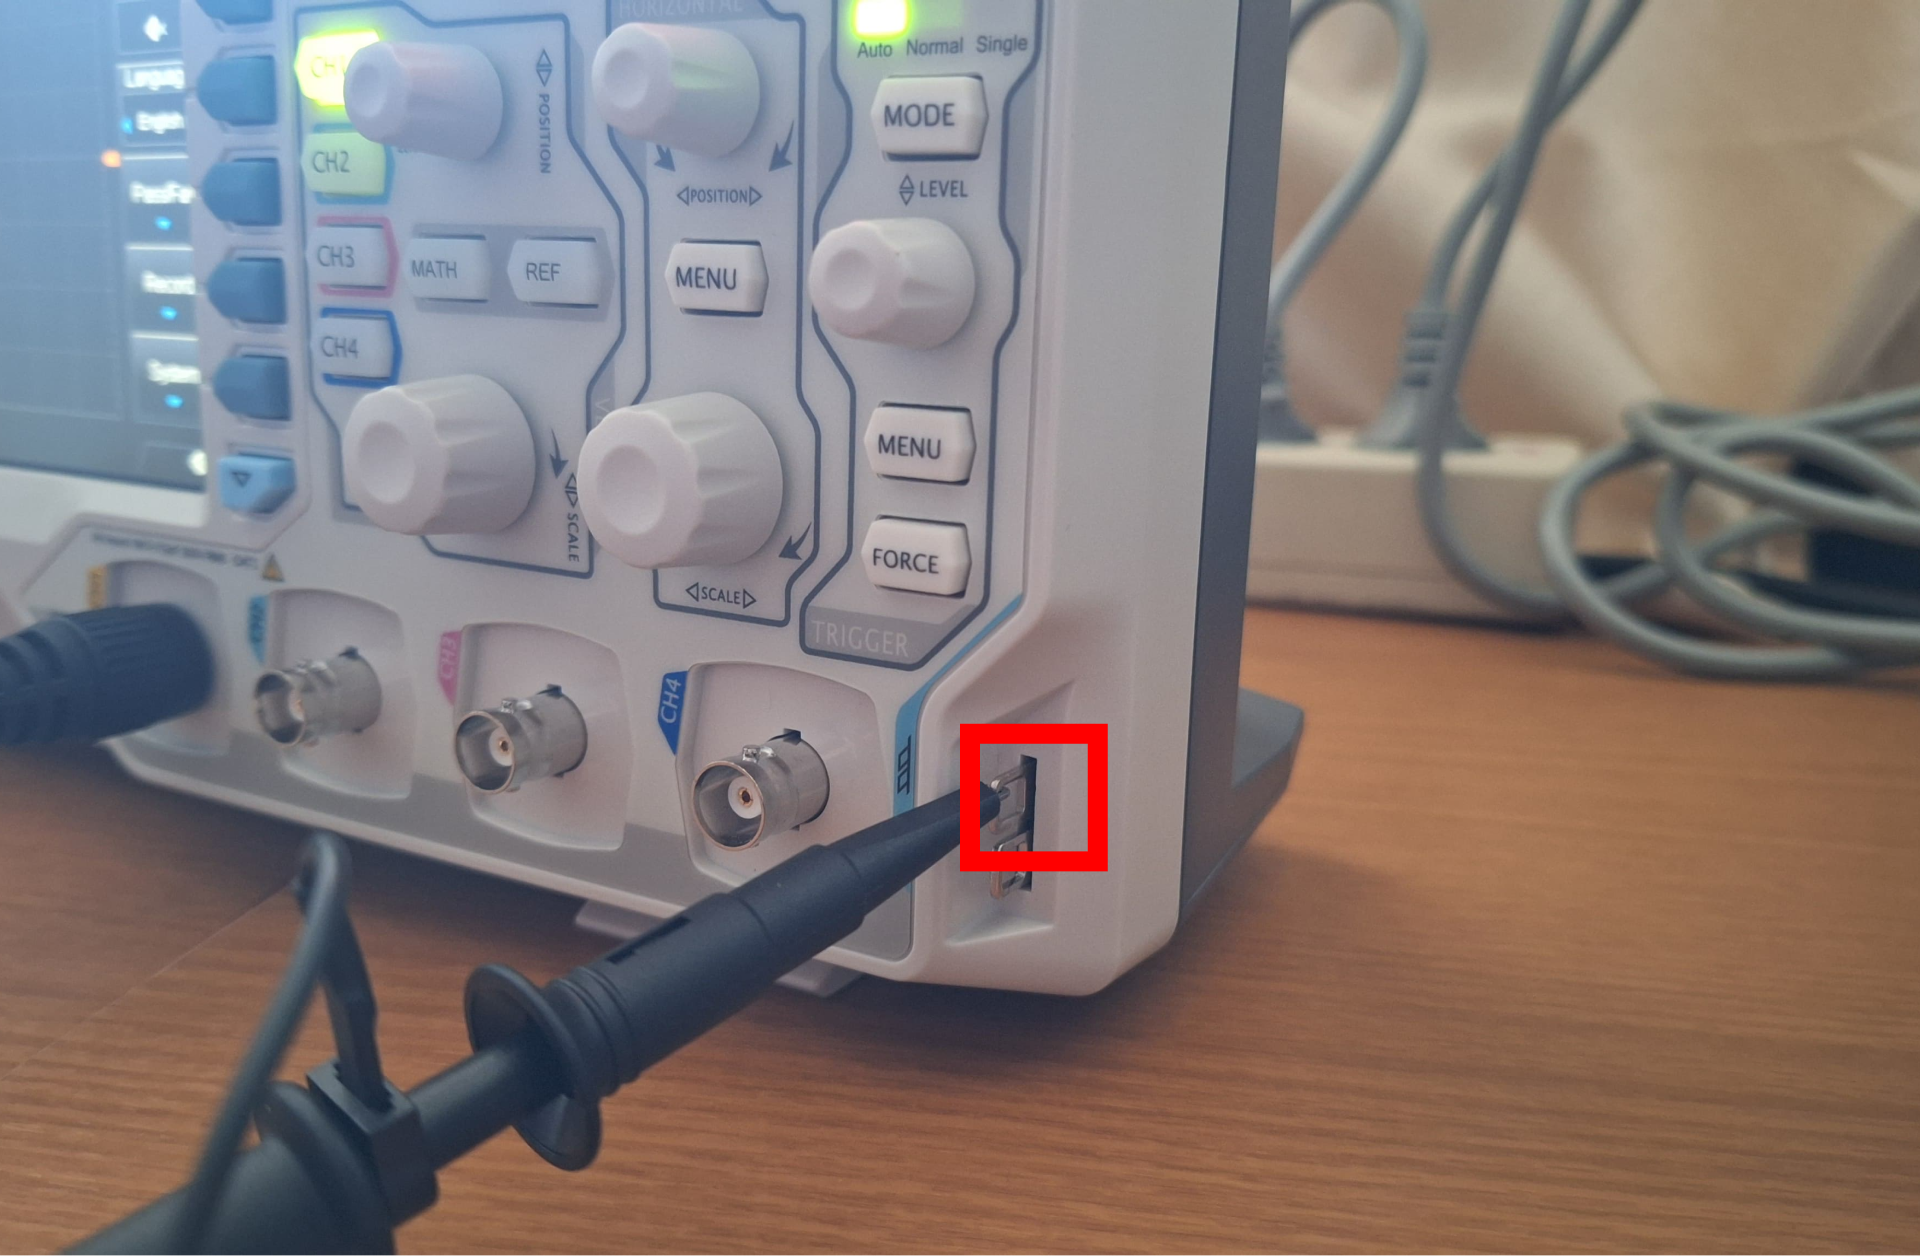
\includegraphics[width=0.8\linewidth]{P1/img/per 1/step 3.png}
				\caption{Step 3}
				\label{fig:Step 3(Group 15)}
			\end{figure}

	\item Tekan tombol AUTO pada osiloskop, lalu sinyal akan muncul setelah kalibrasi.
	\begin{figure}[H]
		\centering
		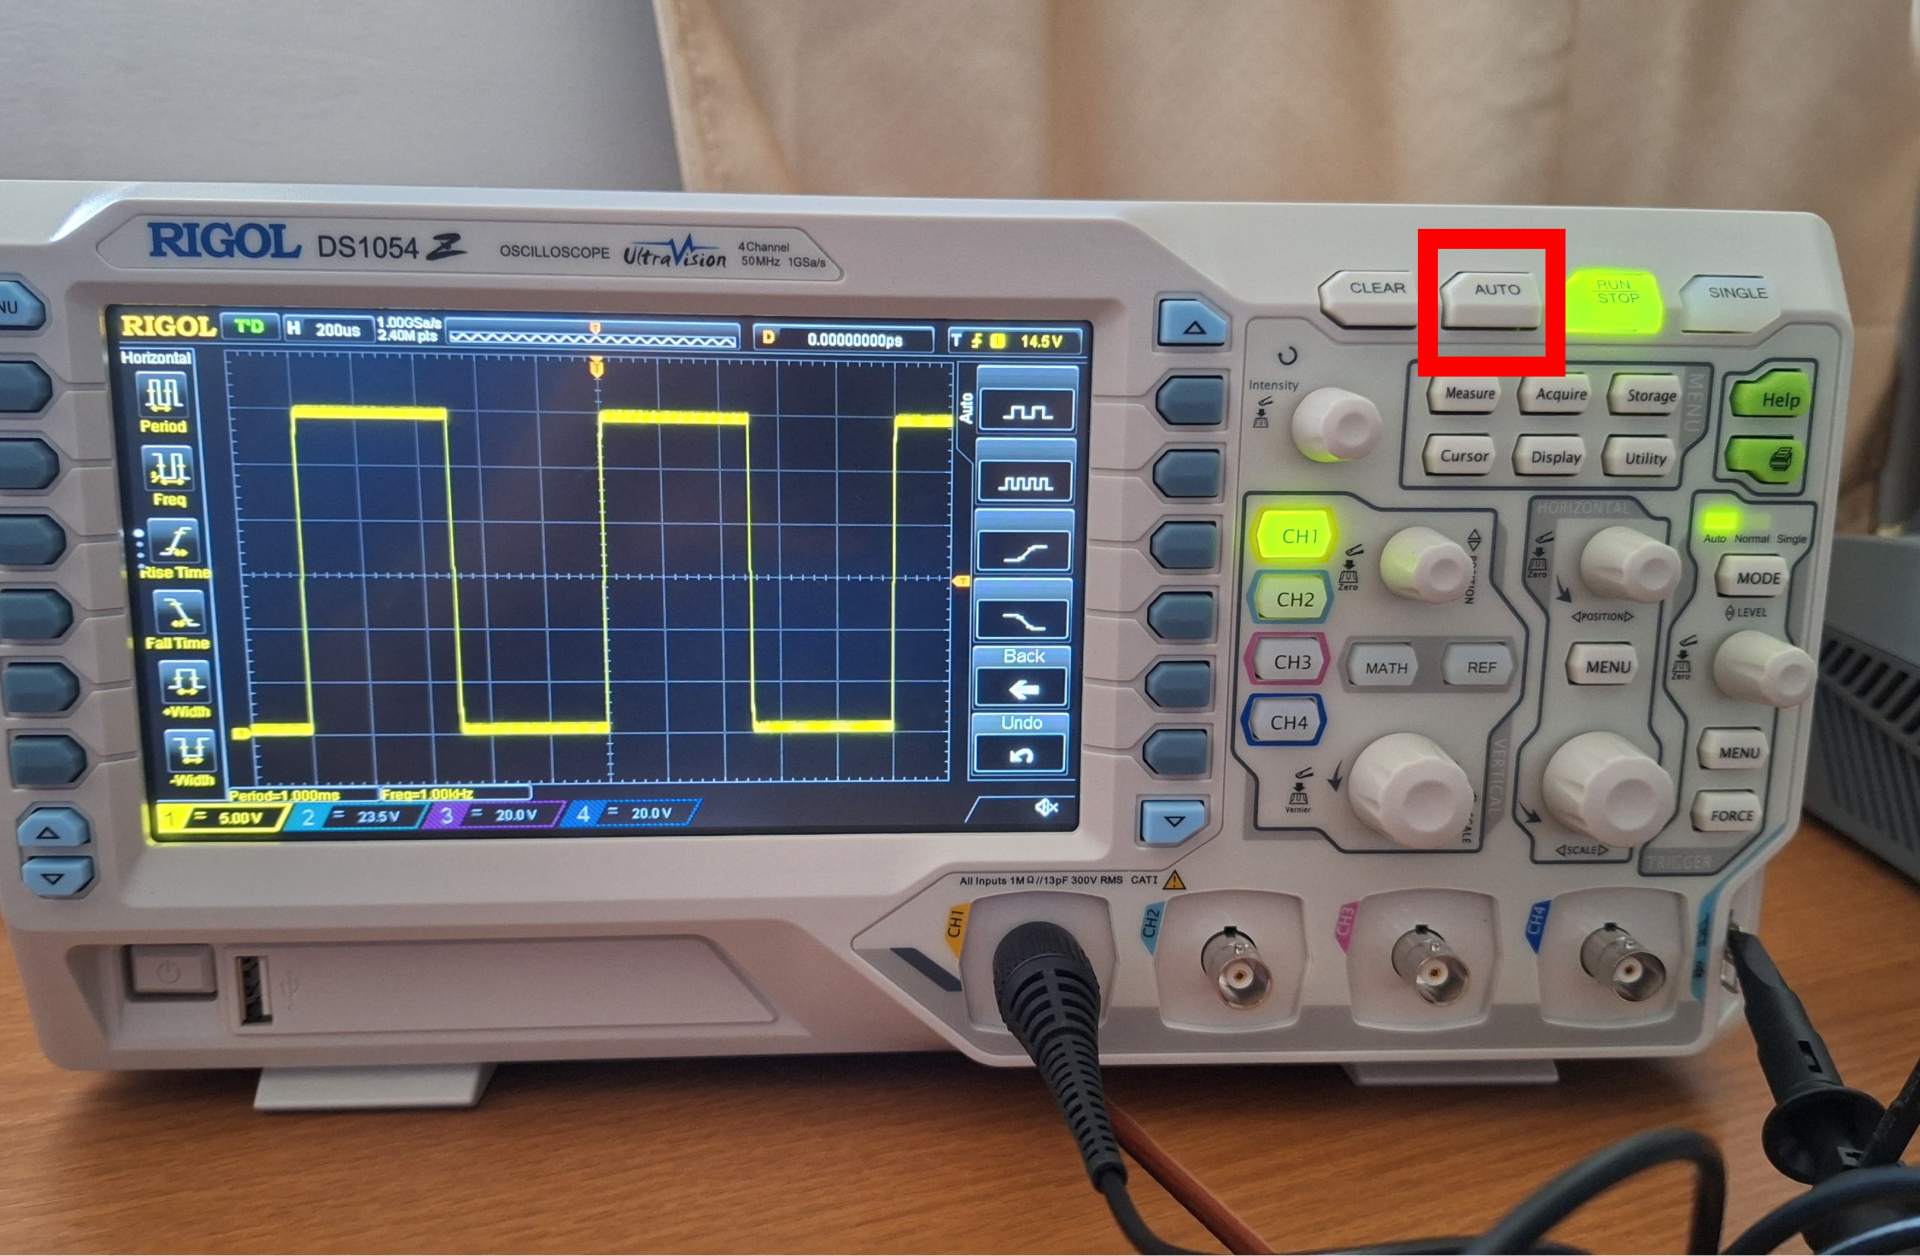
\includegraphics[width=0.8\linewidth]{P1/img/per 1/step 4.png}
		\caption{Step 4}
		\label{fig:Ping Step 4(Group 4)}
	\end{figure}
	\end{enumerate}
\end{center}

%======================PERCOBAAN 2==========================%
\subsection{Percobaan 2}
\begin{center}

	\textbf{Konfigurasi Osiloskop dan Function generator}
	\begin{enumerate}
		\item Hubungkan kabel power ke function generator, lalu tekan tombol power untuk menyalakan Function generator.
		      \begin{figure}[H]
			      \centering
			      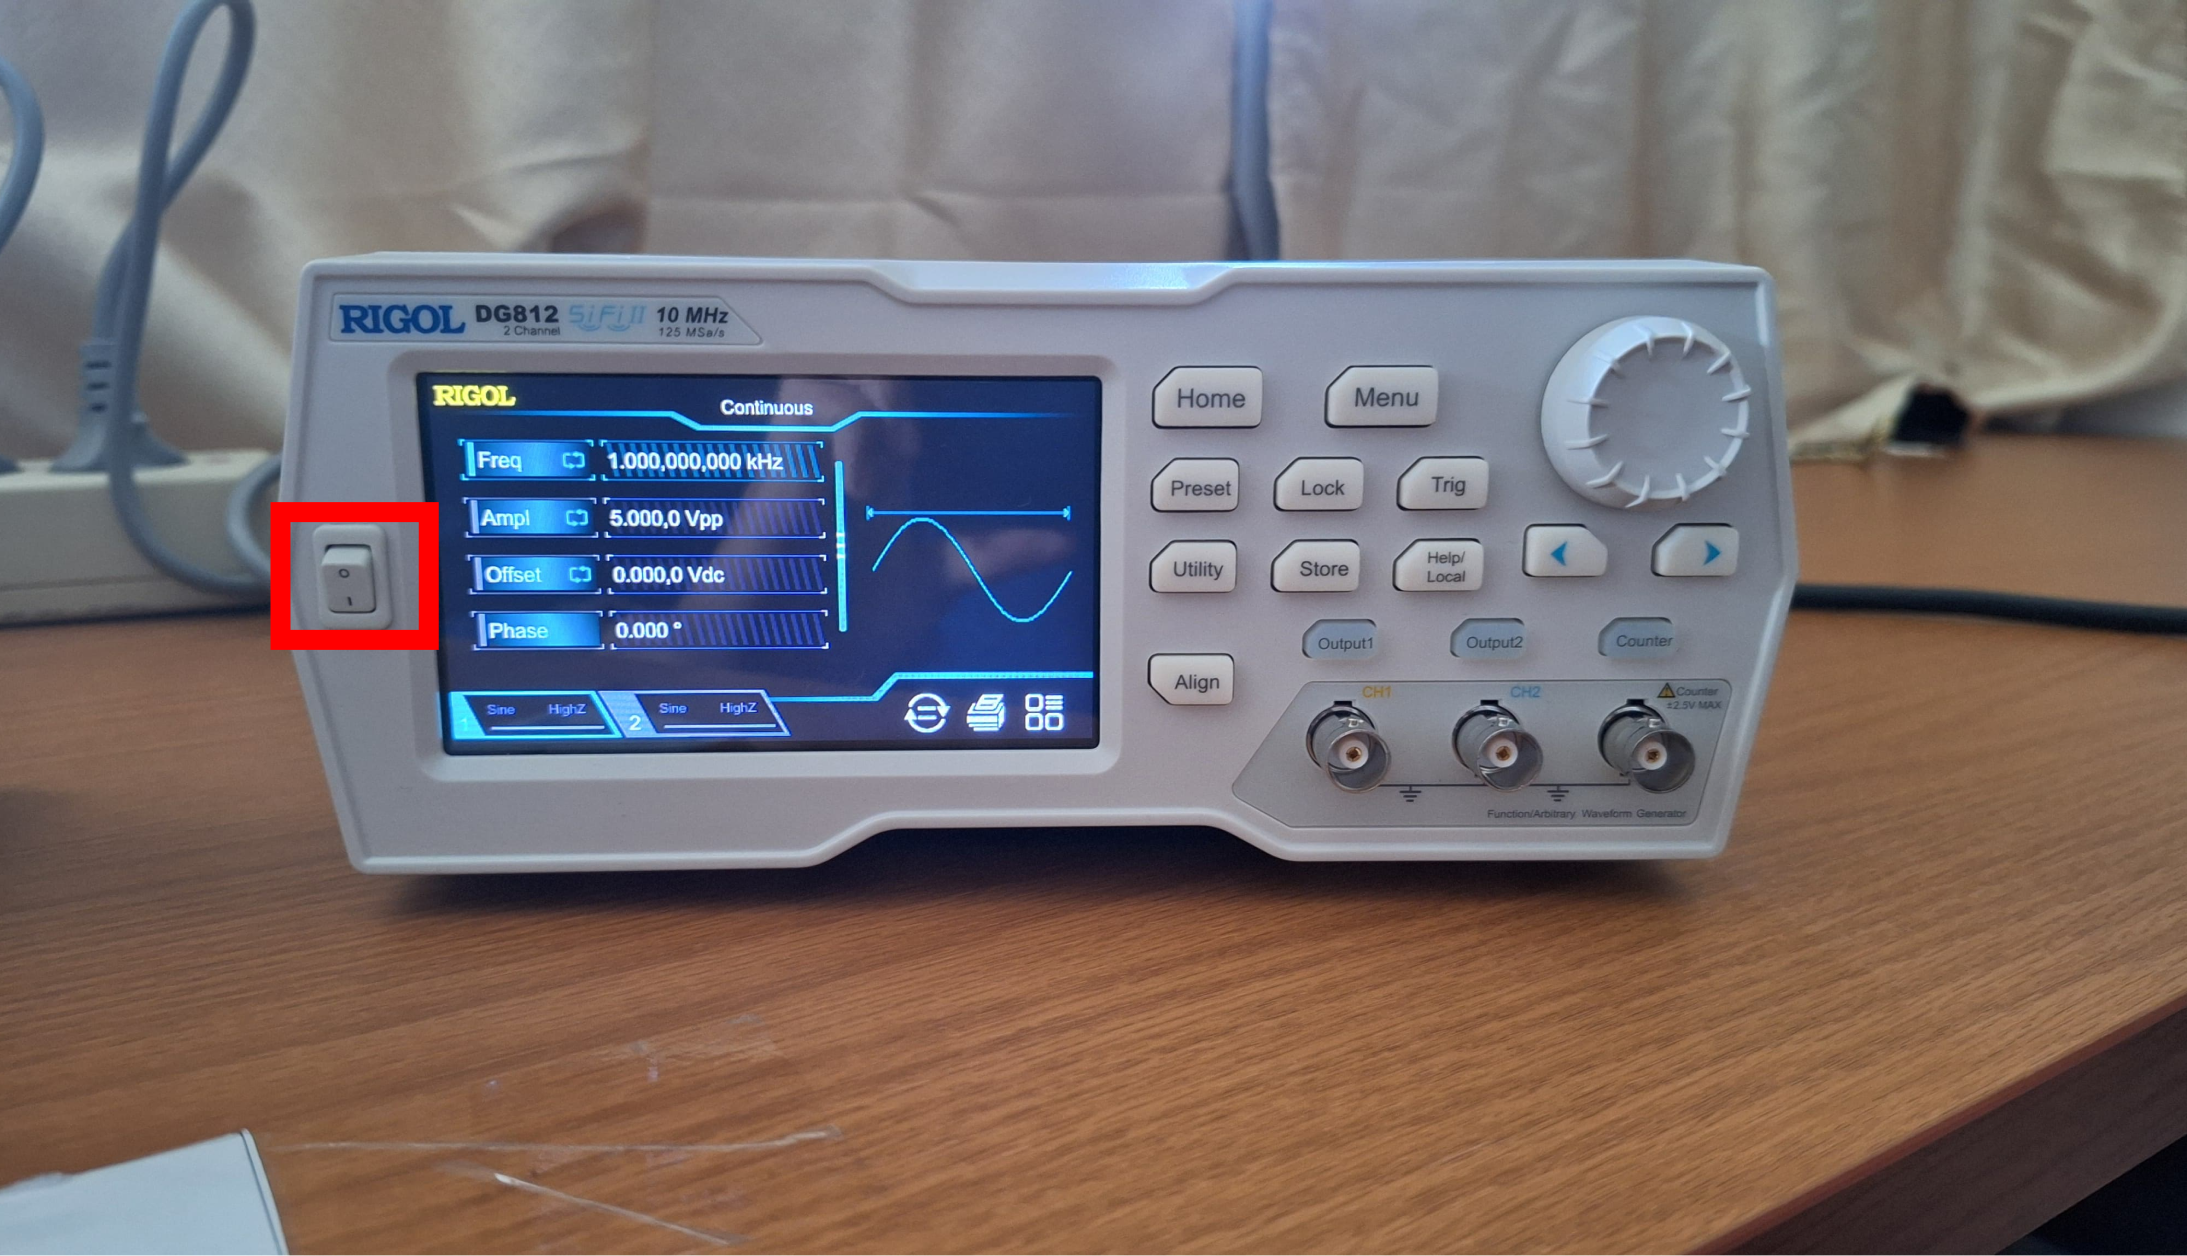
\includegraphics[width=0.8\linewidth]{P1/img/per 2/step 1.png}
			      \caption{Step 1}
			      \label{fig:Step 1(Group 7)}
		      \end{figure}

		\item Hubungkan kabel probe pada channel 1 osiloskop.
		      \begin{figure}[H]
			      \centering
			      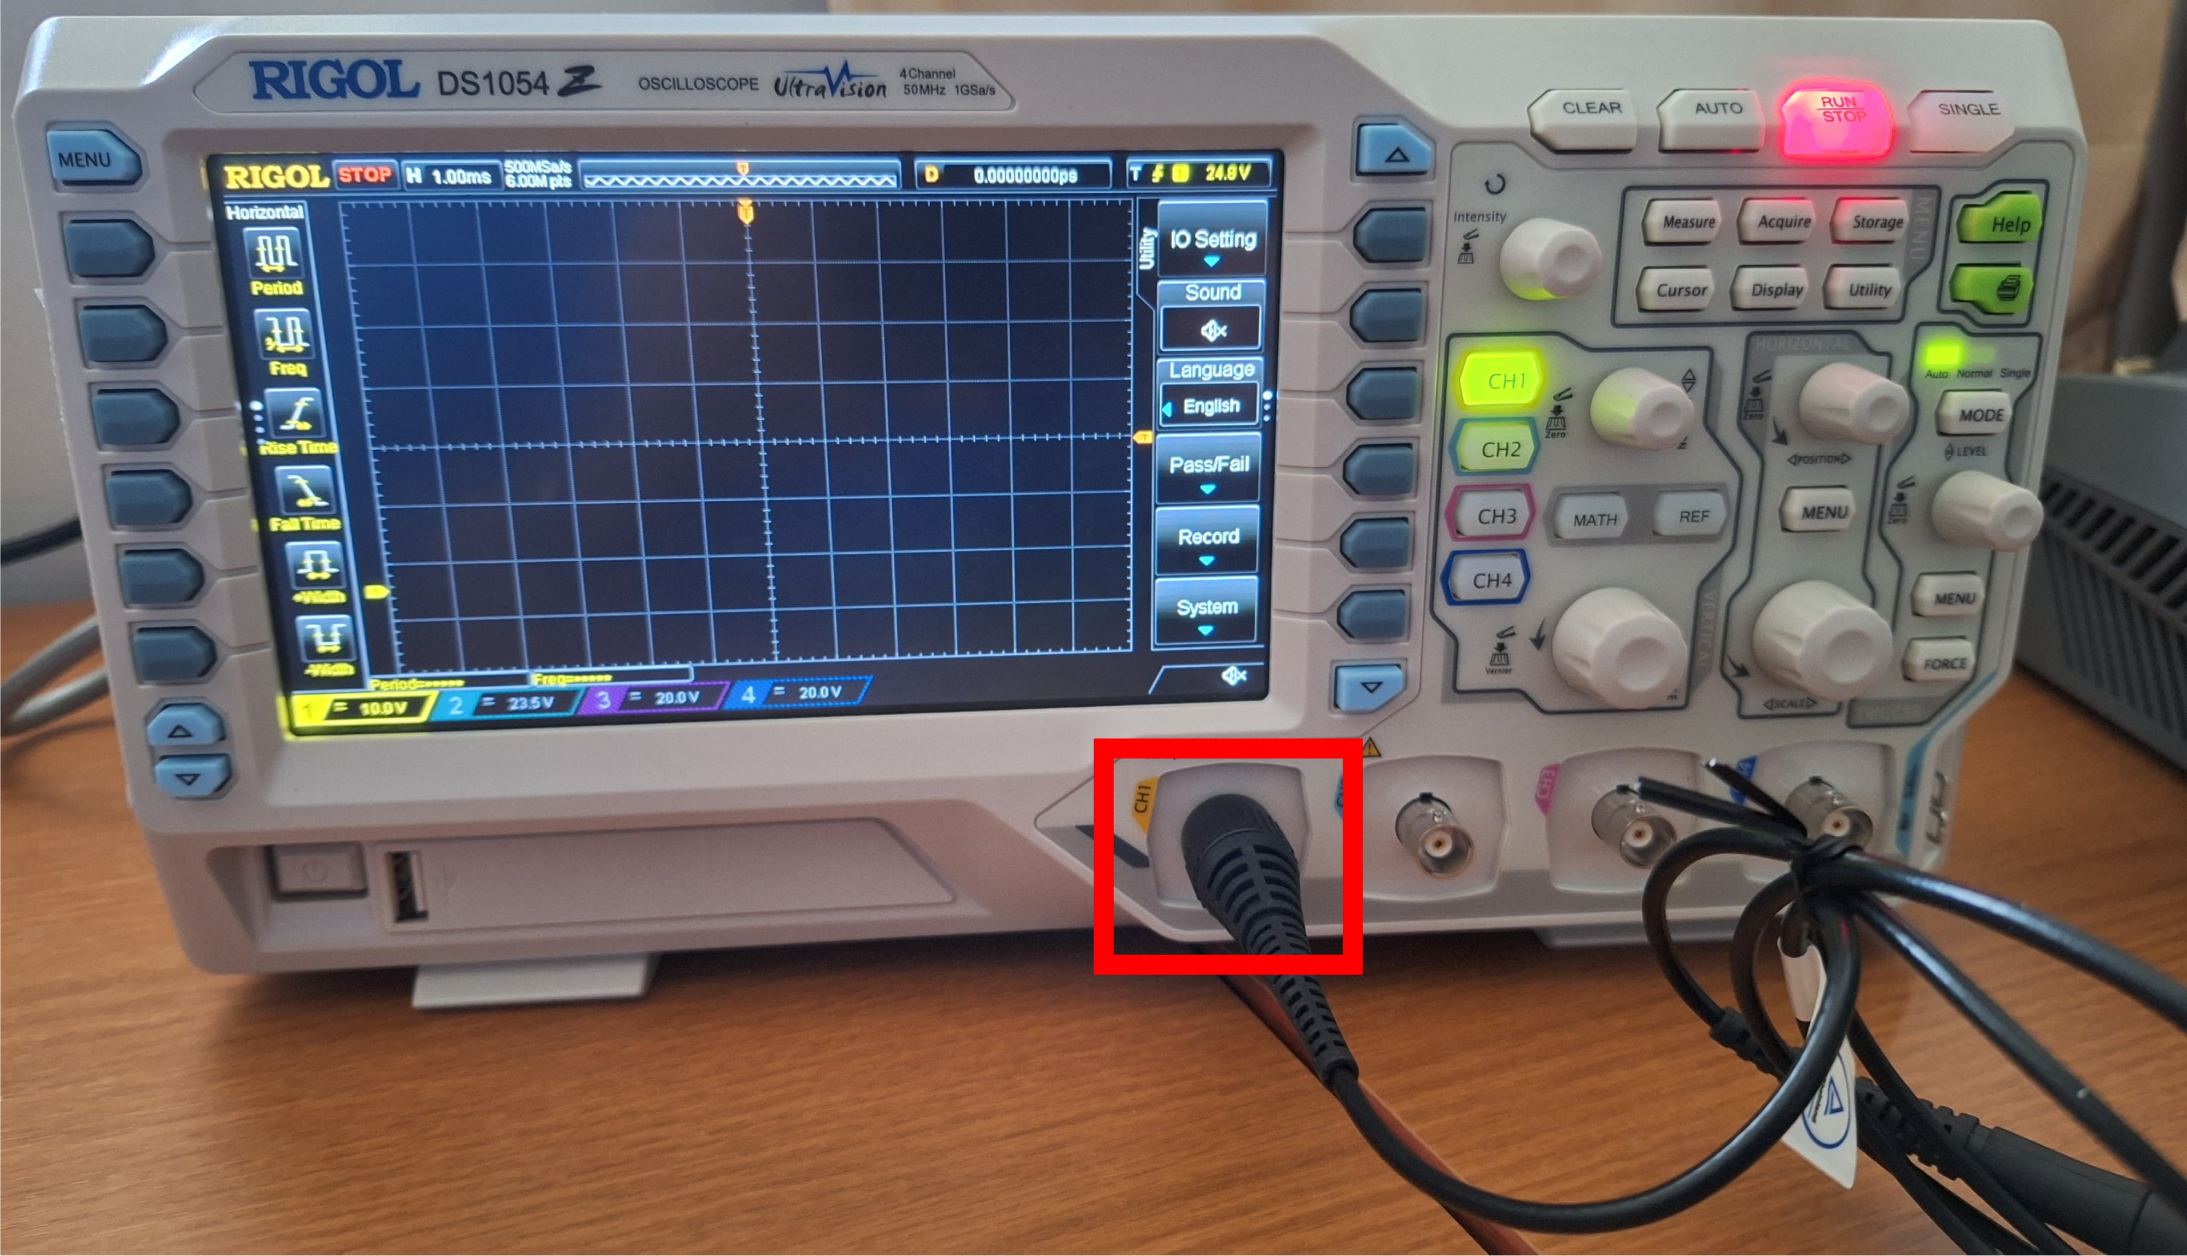
\includegraphics[width=0.8\linewidth]{P1/img/per 2/step 2.png}
			      \caption{Step 2}
			      \label{fig:Step 2(Group 8)}
		      \end{figure}

		\item Hubungkan kabel probe pada output 1 function generator.
		      \begin{figure}[H]
			      \centering
			      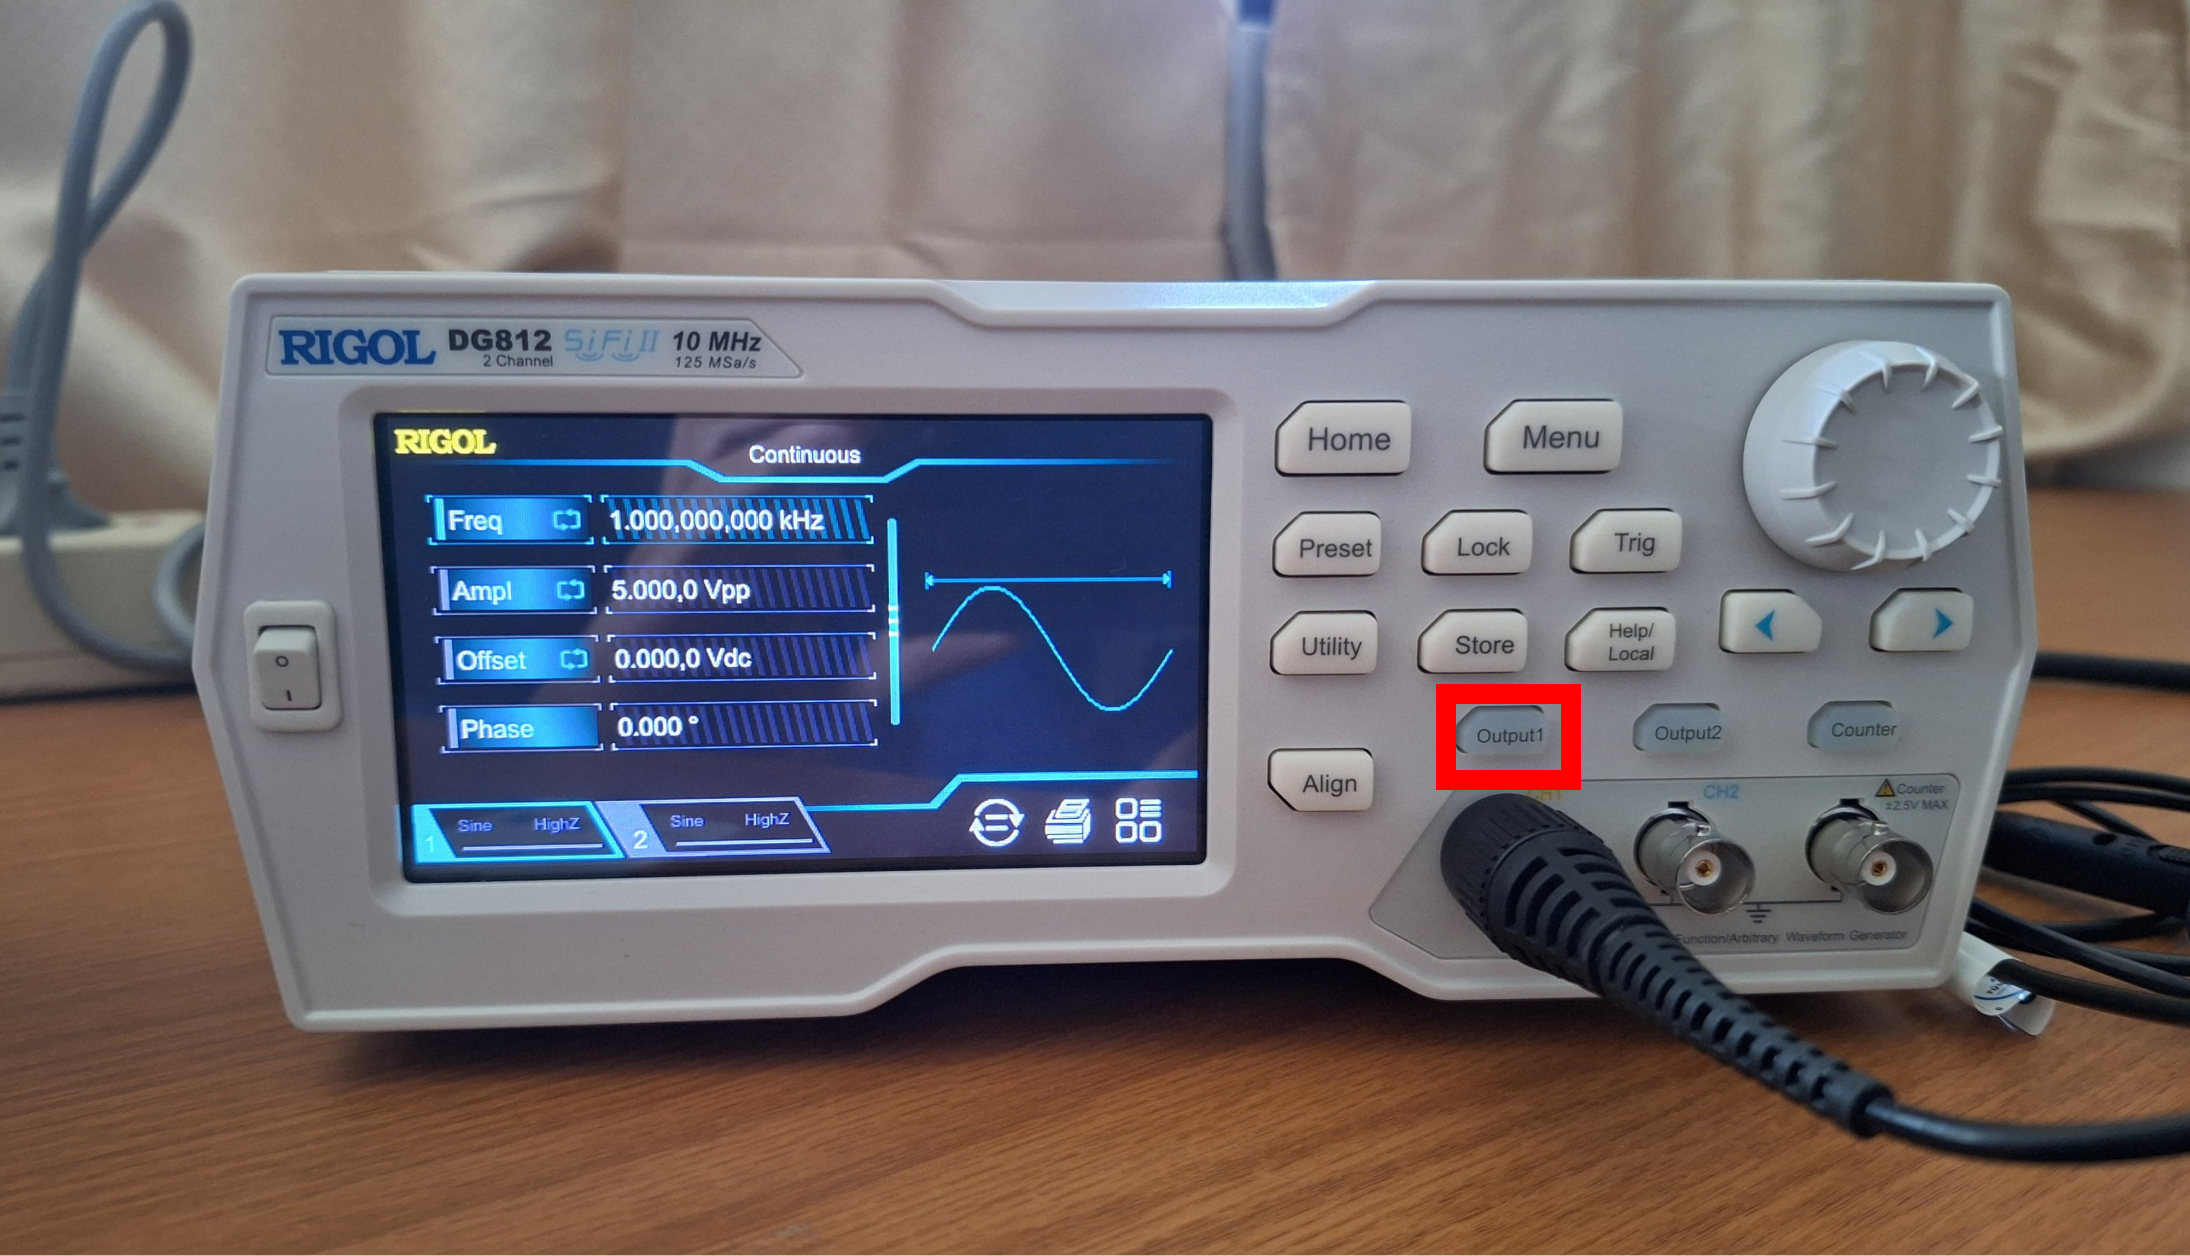
\includegraphics[width=0.8\linewidth]{P1/img/per 2/step 3.png}
			      \caption{Step 3}
			      \label{fig:Step 3(Group 9)}
		      \end{figure}

		\item Hubungkan probe pengait dari osiloskop dan function generator.
		      \begin{figure}[H]
			      \centering
			      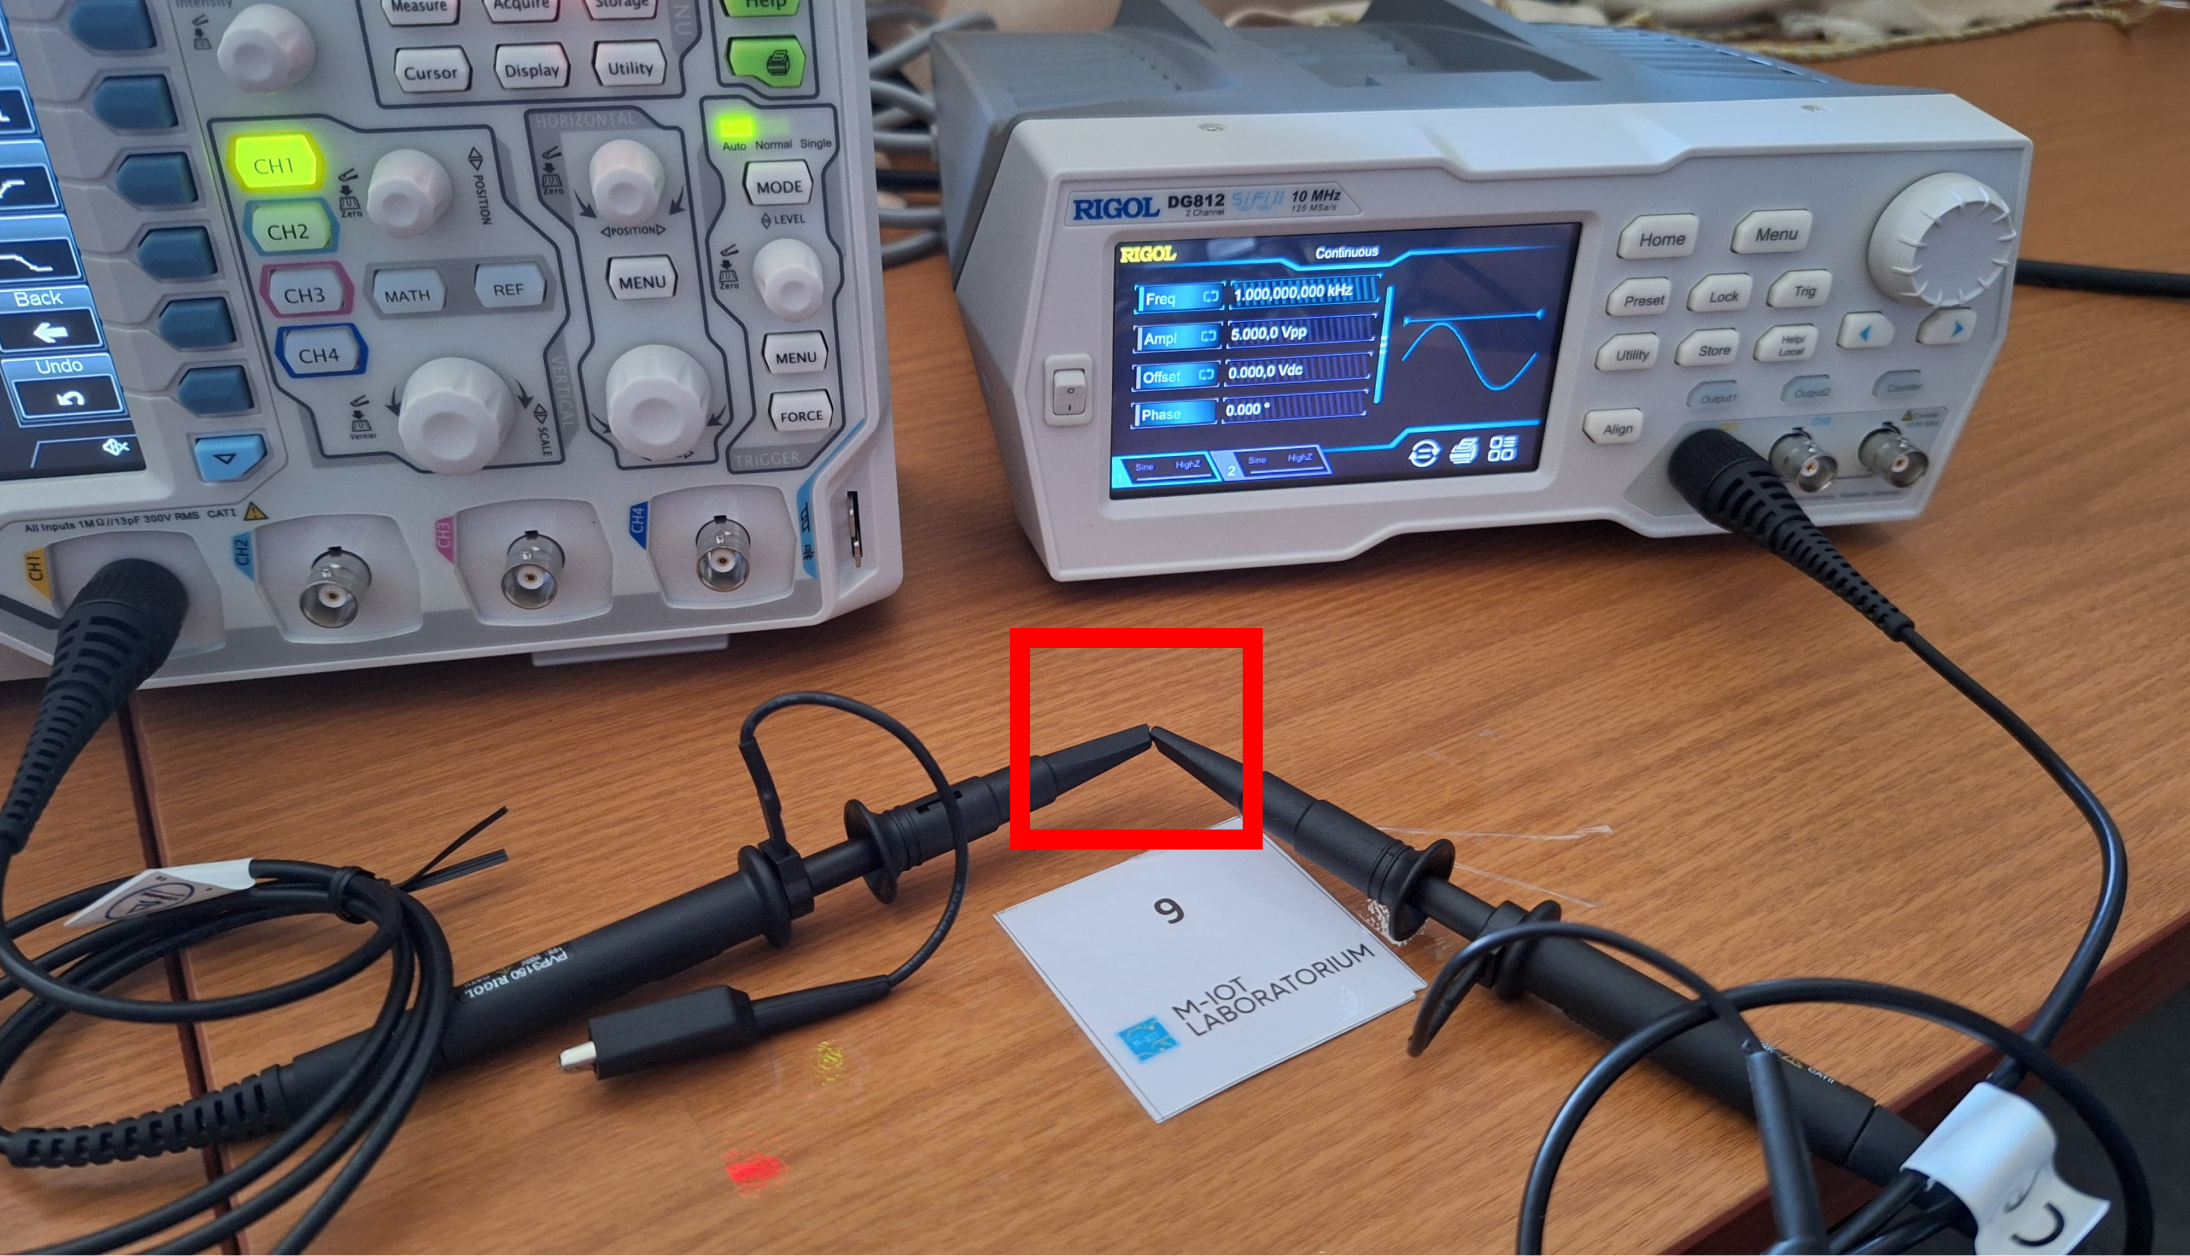
\includegraphics[width=0.8\linewidth]{P1/img/per 2/step 4.png}
			      \caption{Step 4}
			      \label{fig:Step 4(Group 10)}
		      \end{figure}

		\item Tekan tombol output 1 function generator.
		      \begin{figure}[H]
			      \centering
			      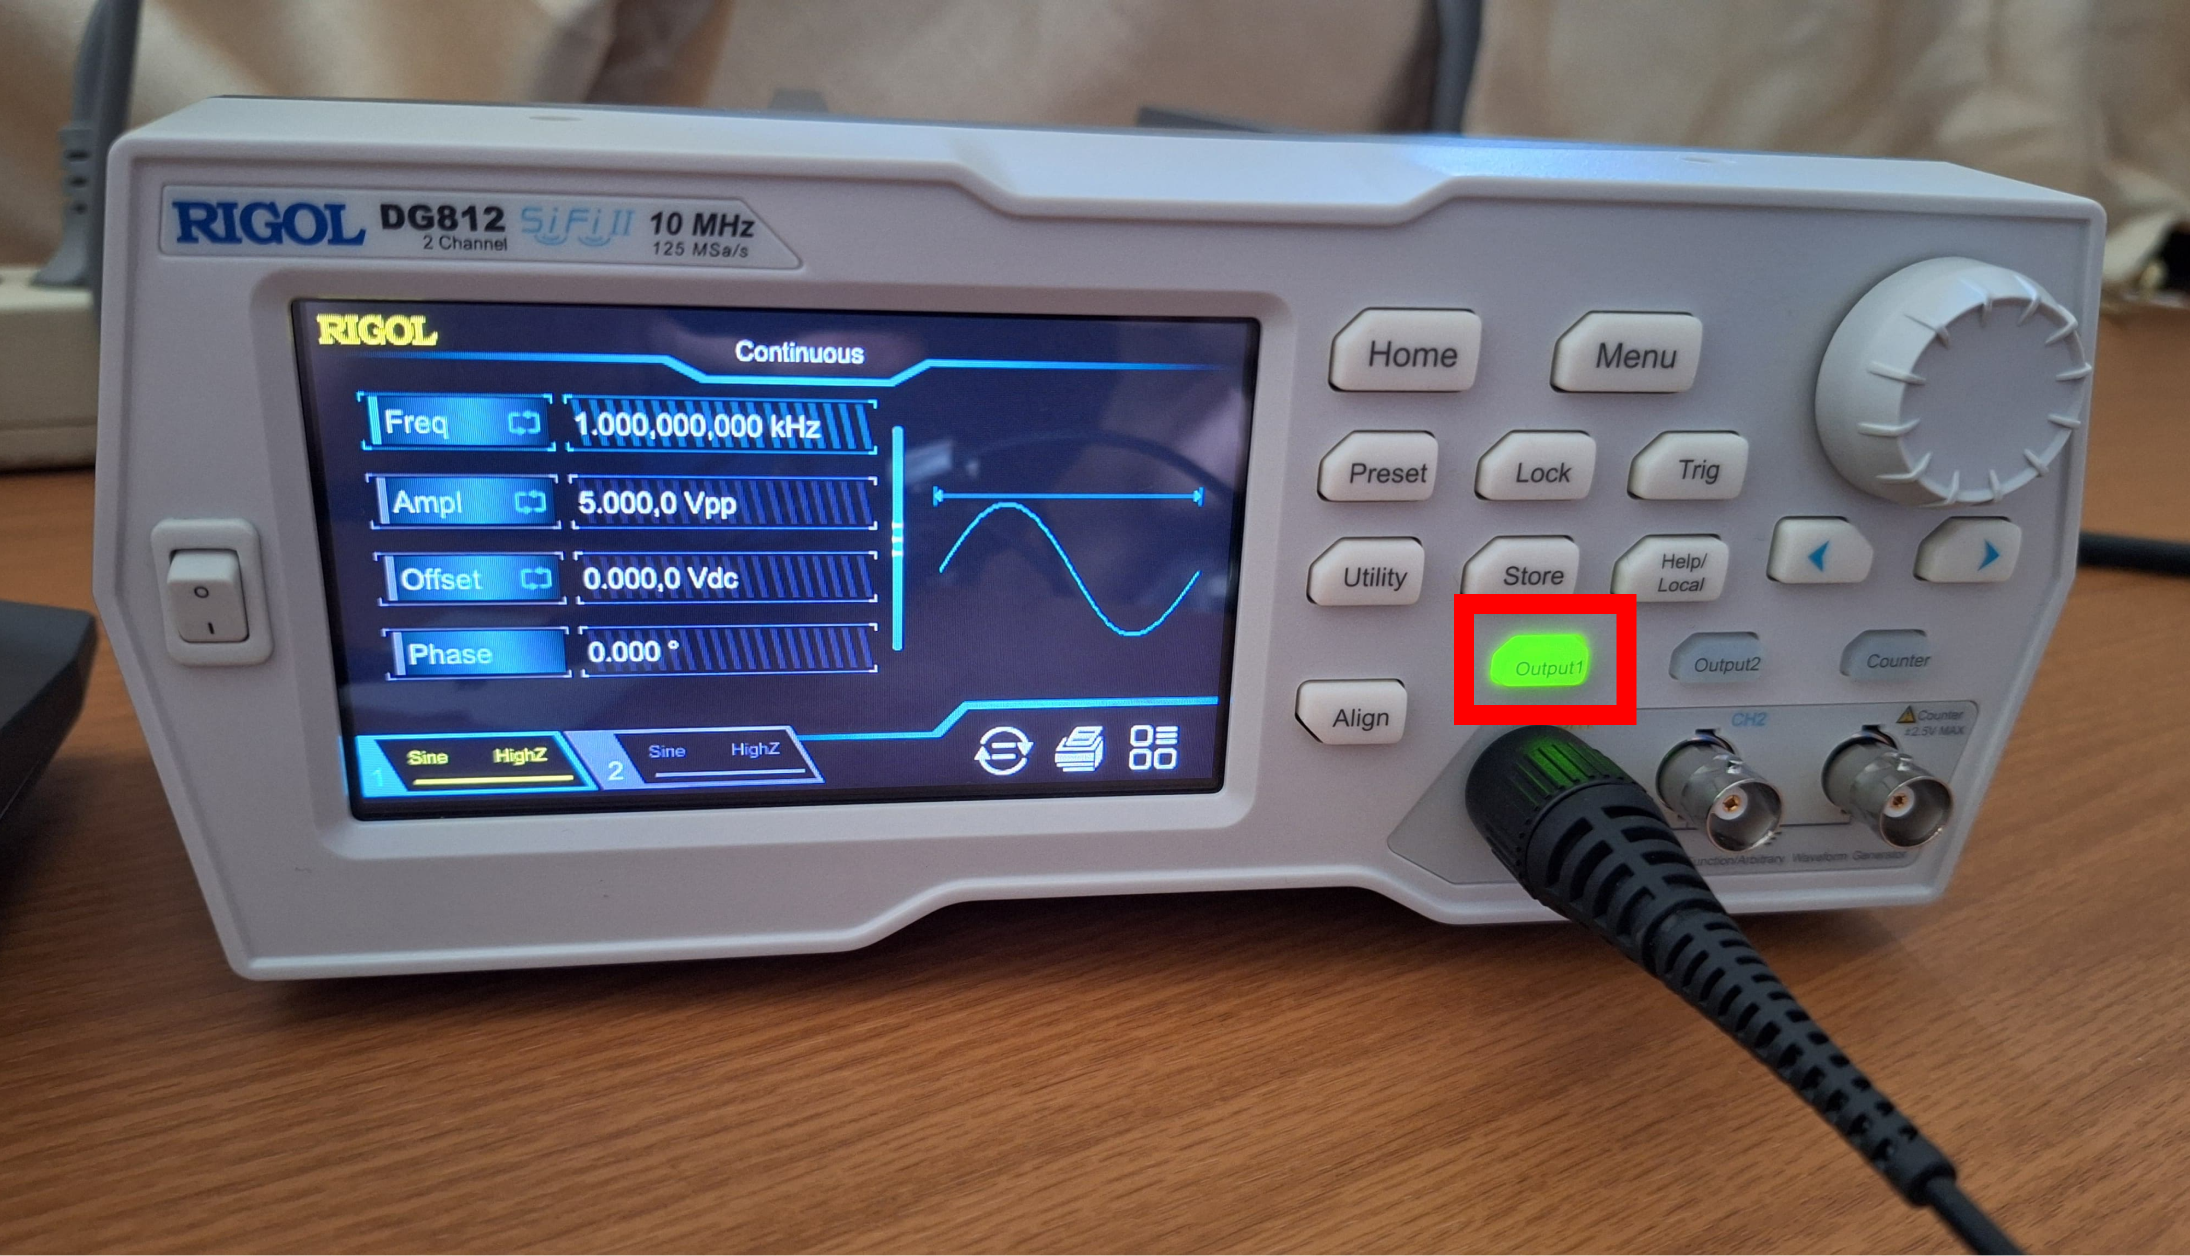
\includegraphics[width=0.8\linewidth]{P1/img/per 2/step 5.png}
			      \caption{Step 5}
			      \label{fig:Step 5(Group 11)}
		      \end{figure}

		\item Tekan tombol AUTO pada osiloskop.
		      \begin{figure}[H]
			      \centering
			      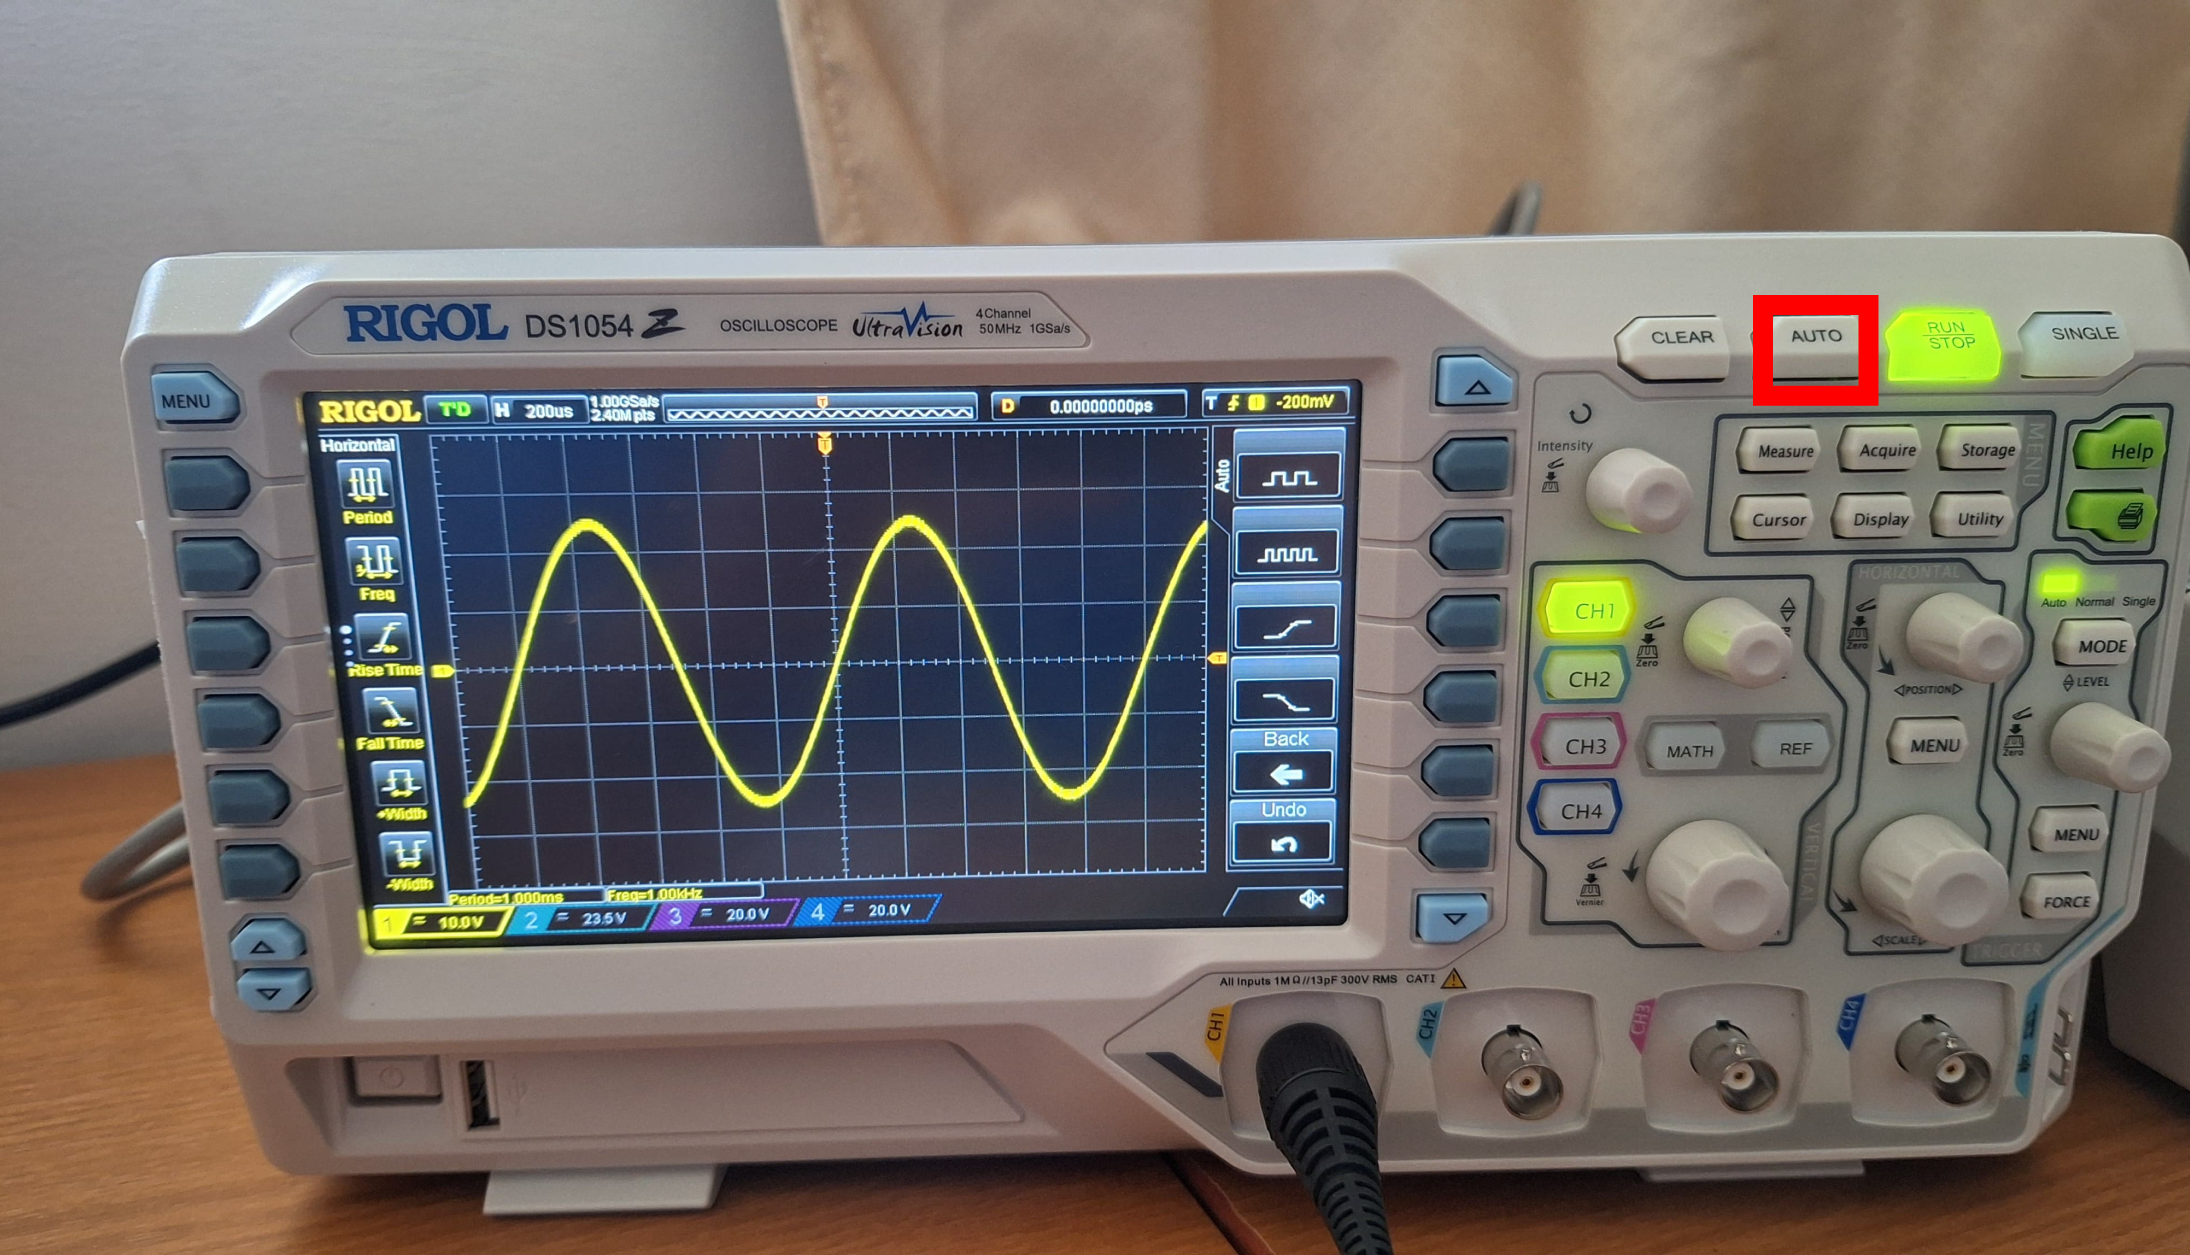
\includegraphics[width=0.8\linewidth]{P1/img/per 2/step 6.png}
			      \caption{Step 6}
			      \label{fig:Step 6(Group 12)}
		      \end{figure}

		\item Matikan output terlebih dahulu setiap ingin mengatur function generator.
		      \begin{figure}[H]
			      \centering
			      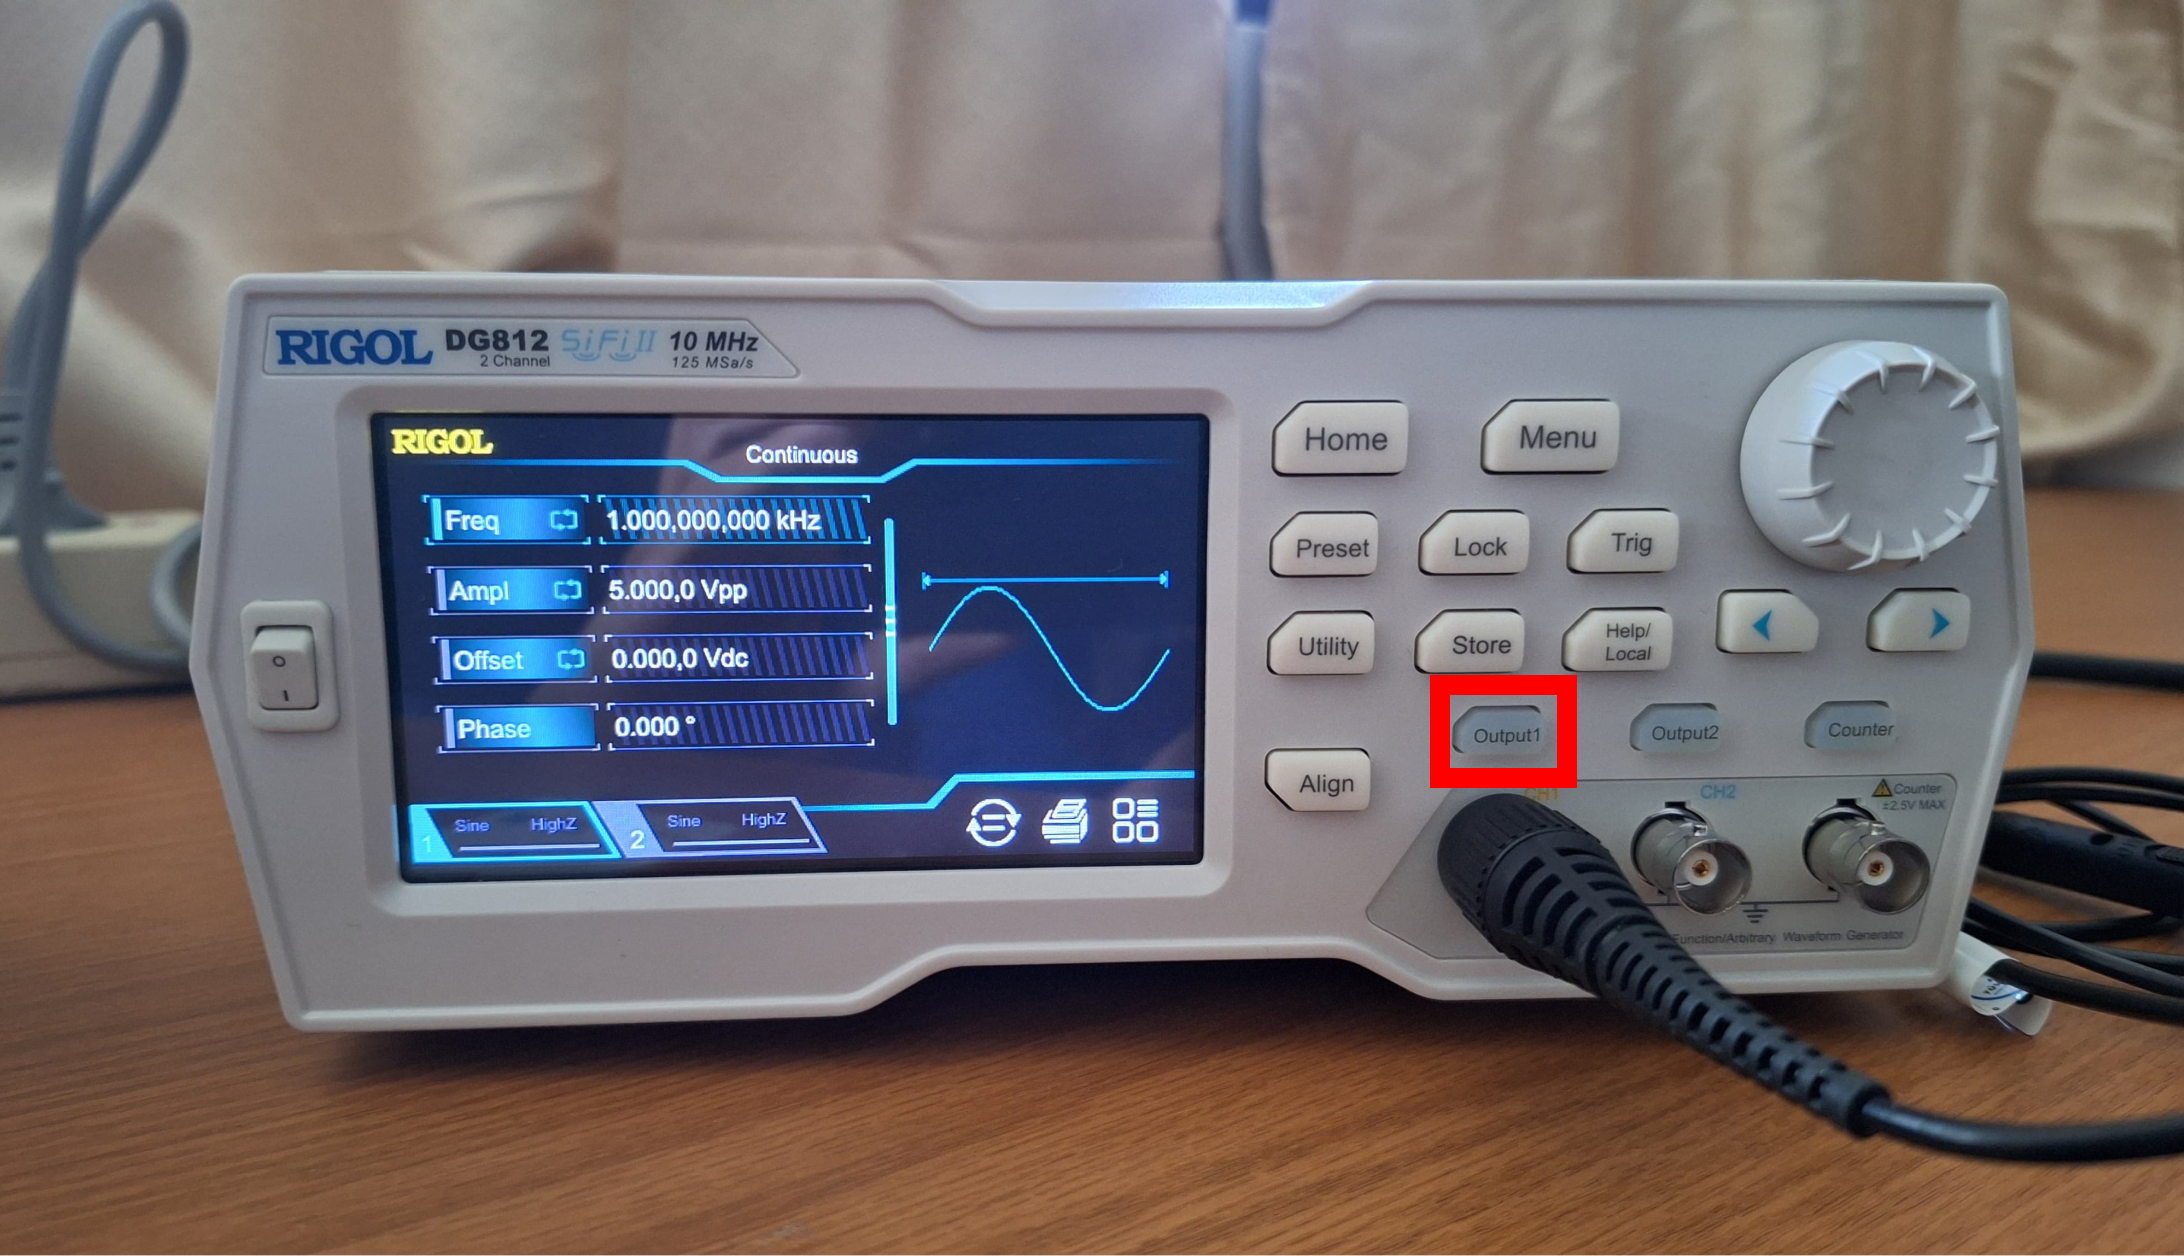
\includegraphics[width=0.8\linewidth]{P1/img/per 2/step 7.png}
			      \caption{Step 7}
			      \label{fig:Step 7(Group 16)}
		      \end{figure}

		\item Tekan tombol Home kemudian ganti ke bentuk sinyal kotak dengan menggunakan 
		\\analog putarnya dan panah kanan/kiri. Jika sudah, tekan analognya untuk klik.
		      \begin{figure}[H]
			      \centering
			      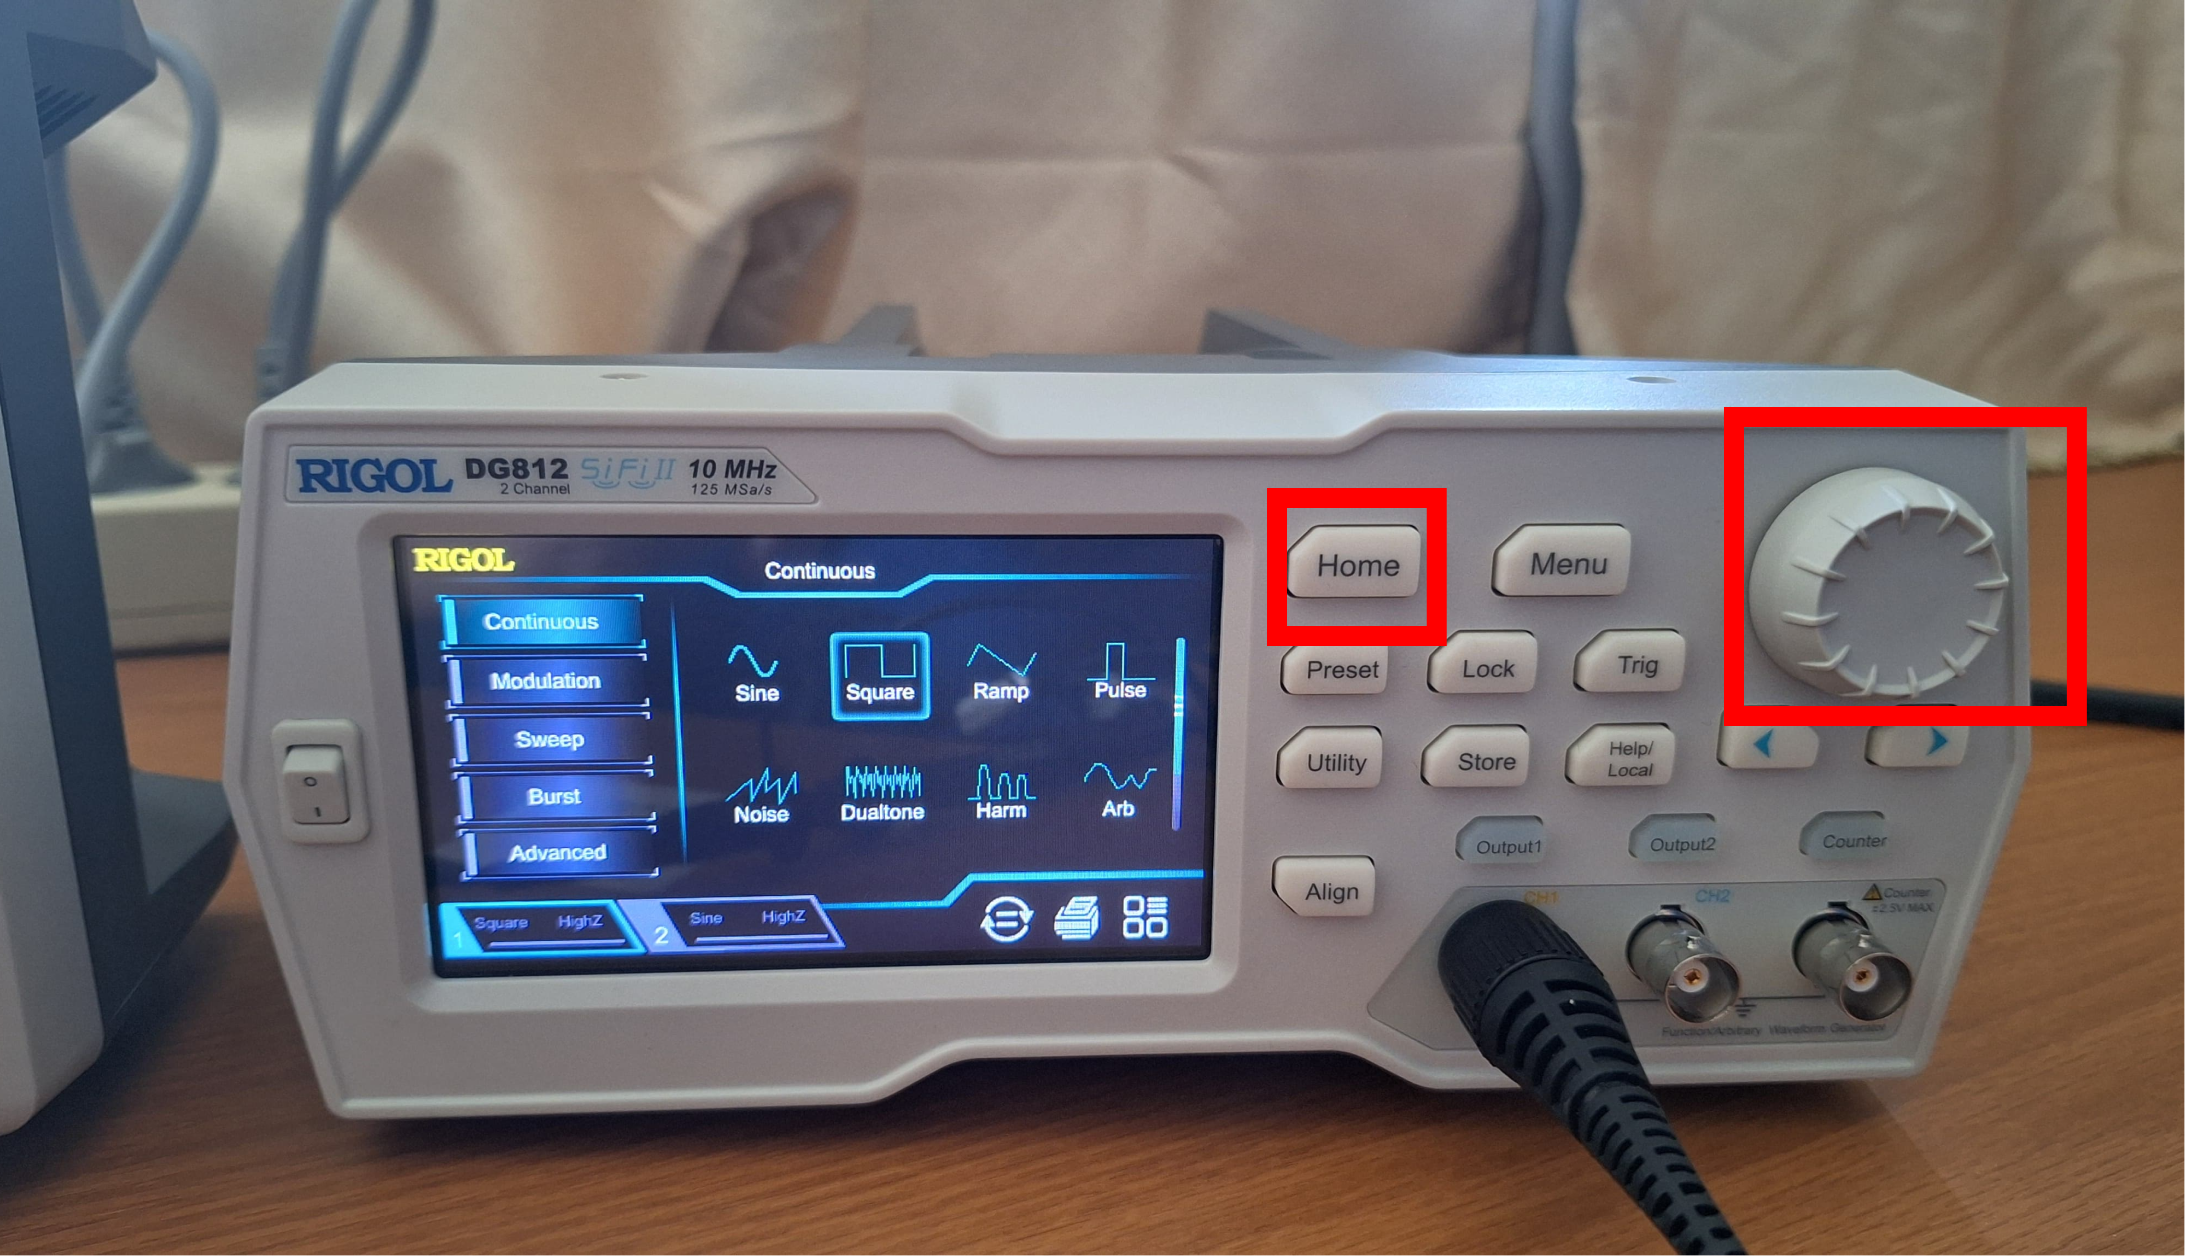
\includegraphics[width=0.7\linewidth]{P1/img/per 2/step 8.png}
			      \caption{Step 8}
			      \label{fig:Step 8(Group 13)}
		      \end{figure}

		\item Tekan Menu untuk kembali, lalu tekan output 1 untuk mengirimkan sinyal ke osiloskop.
		      \begin{figure}[H]
			      \centering
			      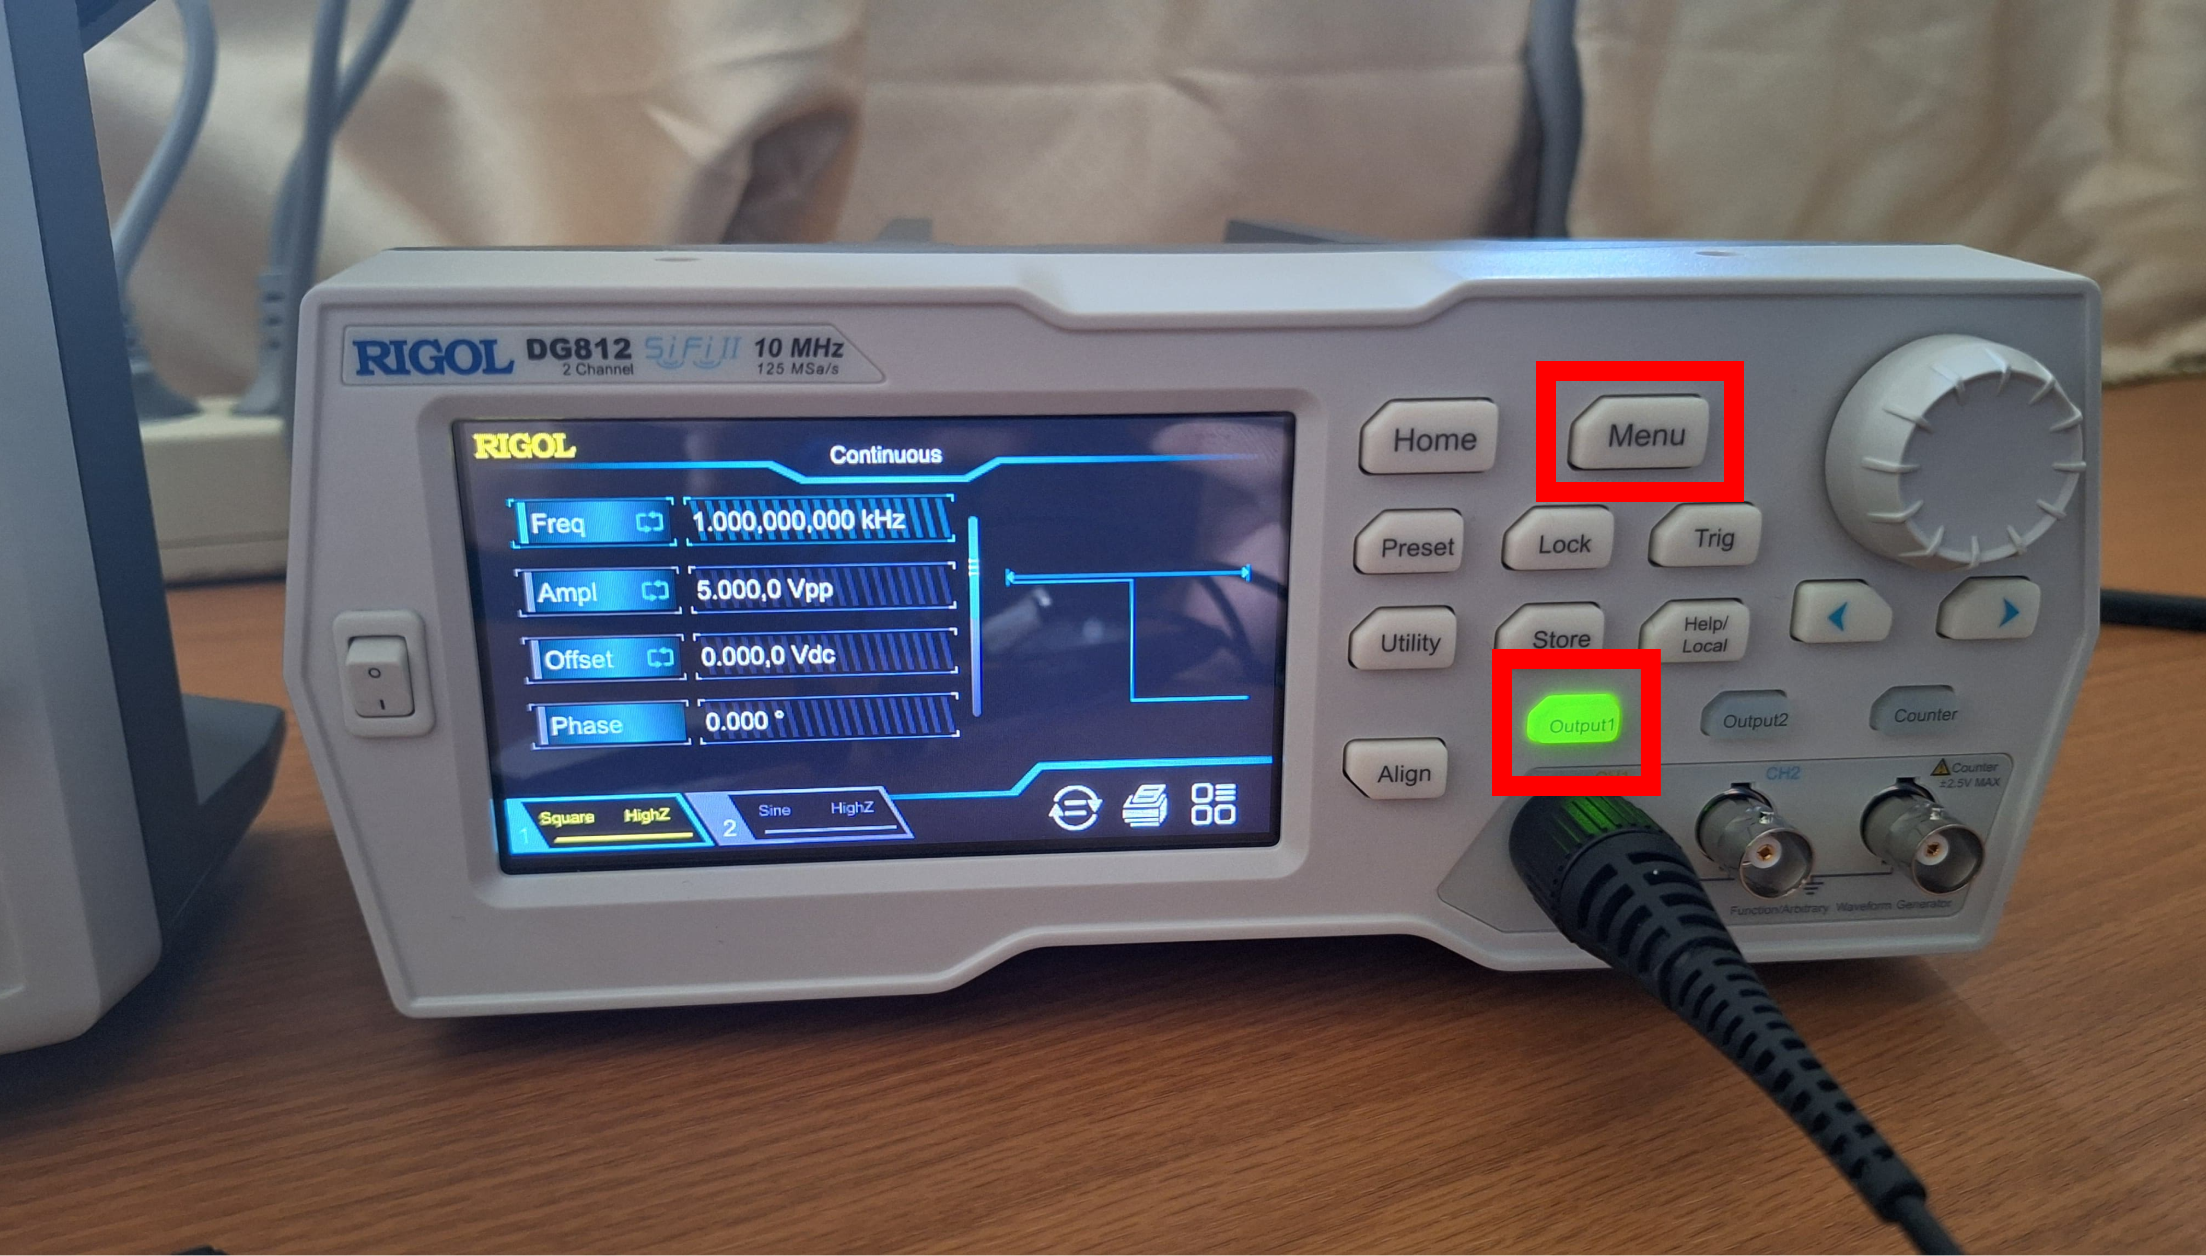
\includegraphics[width=0.7\linewidth]{P1/img/per 2/step 9.png}
			      \caption{Step 9}
			      \label{fig:Step 9(Group 14)}
		      \end{figure}

		\item Tekan AUTO maka sinyal akan ditampilkan melalui osiloskop.
		      \begin{figure}[H]
			      \centering
			      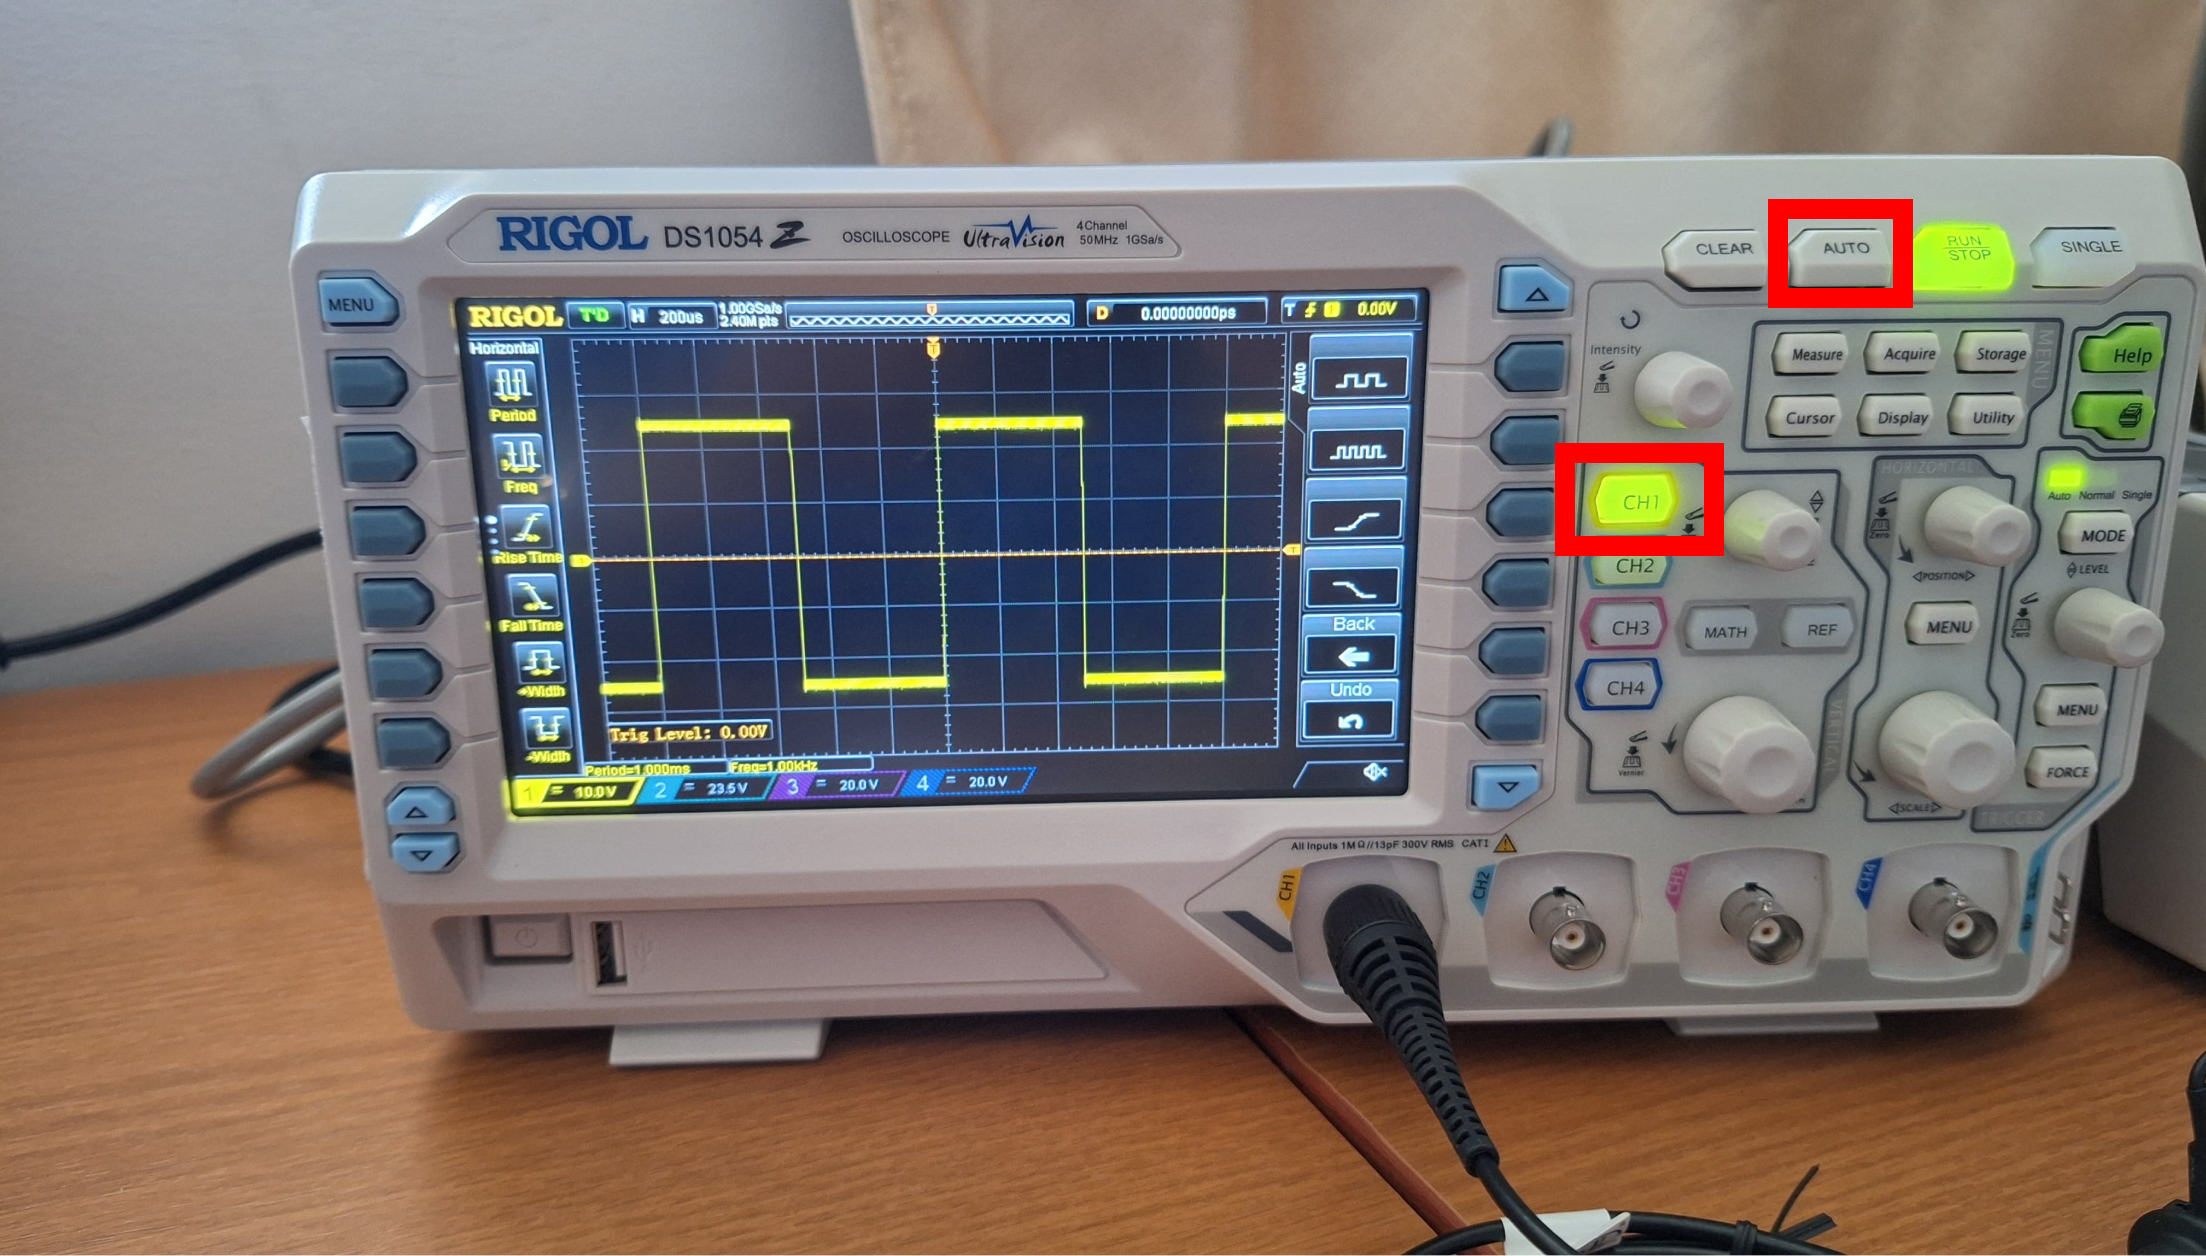
\includegraphics[width=0.7\linewidth]{P1/img/per 2/step 10.png}
			      \caption{Step 10}
			      \label{fig:Step 10(Group 15)}
		      \end{figure}

		\item Lakukanlah kembali untuk menampilkan sinyal arbitary dan sinyal segitiga.
	\end{enumerate}

\end{center}


%===========================================================%
\section{Hasil yang didapat}
Memahami dan mengkonfigurasi Osiloskop dan Function generator dengan tepat.

%===========================================================%
\section{Kesimpulan}
Dengan memahami dan mengkonfigurasi osiloskop dan function generator, kita dapat
\\memahami output sinyal yang ditampilkan oleh osiloskop.
